\documentclass[specialist,
substylefile = spbu.rtx,
               subf,href,colorlinks=true, 12pt]{disser}

%\documentclass[a4paper,12pt]{article}
\usepackage[T2A]{fontenc}
\usepackage[utf8]{inputenc}
\usepackage[english, russian]{babel}
\usepackage[a4paper,
            mag=1000, includefoot,
            left=3cm, right=1.5cm, top=2cm, bottom=2cm, headsep=1cm, footskip=1cm]{geometry}
%\righthyphenmin=2
\ifpdf\usepackage{epstopdf}\fi

% Точка с запятой в качестве разделителя между номерами цитирований
%\setcitestyle{semicolon}

\usepackage{indentfirst}
\usepackage{amsmath}
\usepackage{amssymb}
\usepackage{ dsfont }
\usepackage[table]{xcolor}
\usepackage{graphicx}
\usepackage{vmargin}
\usepackage{wrapfig}
\usepackage{longtable}
\usepackage{footnote}
\usepackage{amsthm}
\usepackage{breqn}
\renewcommand{\baselinestretch}{1.5}
\usepackage{amsfonts}
\usepackage[hidelinks]{hyperref}
\usepackage{listings}
\usepackage{subcaption}
\usepackage{mathtools}
\usepackage{xcolor}
\usepackage{algorithm}
\usepackage{algpseudocode}

%New colors defined below
\definecolor{codegreen}{rgb}{0,0.6,0}
\definecolor{codegray}{rgb}{0.5,0.5,0.5}
\definecolor{codepurple}{rgb}{0.58,0,0.82}
\definecolor{backcolour}{rgb}{0.95,0.95,0.92}

\lstdefinestyle{mystyle}{
  backgroundcolor=\color{backcolour}, commentstyle=\color{codegreen},
  keywordstyle=\color{magenta},
  numberstyle=\tiny\color{codegray},
  stringstyle=\color{codepurple},
  basicstyle=\ttfamily\footnotesize,
  breakatwhitespace=false,         
  breaklines=true,                 
  captionpos=b,                    
  keepspaces=true,                 
  numbers=left,                    
  numbersep=5pt,                  
  showspaces=false,                
  showstringspaces=false,
  showtabs=false,                  
  tabsize=2
}
\setcounter{tocdepth}{2}

\graphicspath{{fig/}}

\lstset{style=mystyle}
\addto\captionsrussian{\def\refname{Список литературы}}
\DeclareMathOperator{\spdepth}{spdepth}
\DeclareMathOperator{\odepth}{odepth}
\DeclareMathOperator{\sign}{sign}
\DeclareMathOperator*{\med}{med}

\newtheorem{theorem}{Теорема}
\newtheorem{corollary}{Следствие}
\newtheorem{proposition}{Предложение}
\newtheorem{lemma}{Лемма}

\floatname{algorithm}{Алгоритм}
    
\begin{document}

  \institution{%
    Санкт-Петербургский государственный университет
}

\title{Выпускная квалификационная работа}

% Тема
\topic{Исследование одной робастной оценки}

% Автор
\author{\textsc{Филатова} Арина Алексеевна}

\group{%
    Уровень образования: бакалавриат\\
    Направление 01.03.02 <<Прикладная математика и информатика>>\\
    Основная образовательная программа СВ.5004.2020 <<Прикладная математика и информатика>>
}

% Научный руководитель
\sa       {M.\,C.~Ермаков}
\sastatus {Профессор, кафедра статистического моделирования\,\\
           д.\,ф.-м.\,н., профессор}

% Рецензент
\rev      {В.\,Н.~Солев}
\revstatus{Старший научный сотрудник, Петербургское отделение математического института РАН, лаборатория статистических методов}

% Город и год
\city{Санкт-Петербург}
\date{\number\year}

\maketitle

%%
%% Titlepage in English
%%
%
\institution{%
    Saint Petersburg State University \\
    Applied Mathematics and Computer Science
}
%
\title{Graduation Project}
%
%% Topic
\topic{Investigation of one robust estimator
}
%
%% Author
\author{\textsc{Filatova} Arina Alekseevna} % Full Name
\group{}

%% Scientific Advisor
\sa       {M.\,S.~Ermakov}
\sastatus {Professor, Department of Statistical Modelling}
%
%% Reviewer
\rev      {V.\,N.~Solev}
\revstatus{Senior research associate}
%
%% City & Year
\city{Saint Petersburg}
\date{\number\year}

\maketitle[en]

\tableofcontents

\newpage

\chapter{Введение}

При исследовании данных явно или неявно приходится делать ряд допущений. Статистические методы, основанные на определенных предположениях о распределении данных, называют классическими. К ним относятся, например, выборочное среднее, стандартное отклонение и выборочная дисперсия. Эти методы работают хорошо, когда предположения выполняются, однако в реальных данных часто встречаются аномалии, выбросы и другие искажения, которые могут значительно влиять на результаты анализа, делая их ненадежными.

Робастные статистические методы, напротив, разработаны для обеспечения устойчивости оценок и выводов и обладают слабой чувствительностью к
малым отклонениям от предположений. Они менее подвержены влиянию выбросов и обеспечивают более надежные результаты в ситуациях, когда классические методы могут оказаться неприменимыми. Одним из ключевых преимуществ робастных методов является их способность эффективно обрабатывать данные, которые не соответствуют идеализированным предположениям.

%Существует несколько возможных интерпретаций понятия <<малые отклонения>>. Примером таких отклонений являются выбросы --- значения, которые сильно отличаются от остальных наблюдений. Может быть и иная ситуация: резко выделяющихся наблюдений нет, но сами данные повреждены, например, из-за округления при их записи.

%Исследование робастных методов оценивания имеет важное значение для статистического анализа и принятия решений в различных областях.

Известно, что многие обобщения медианы на многомерный случай являются робастными \cite{Robust}. Зная ее, можно делать выводы о характеристиках данных, описывать их, интерпретировать и принимать решения на их основе. Поэтому исследования робастных оценок многомерных медиан представляют собой актуальную задачу, поскольку эти оценки являются важным инструментом не только для статистического анализа, но и для принятия решений в различных областях науки и бизнеса.
\vspace{2ex}

\textbf{Цель выпускной работы:}

Исследовать новый робастный алгоритм для оценки многомерного параметра положения, который можно считать некоторым обобщением медианы на многомерный случай, уделяя особое внимание его сходимости, временной сложности и робастности. 

\newpage

\textbf{Задачи выпускной работы:}

\begin{itemize}
    \item Ознакомление с ключевыми понятиями робастного оценивания и особенно 
робастного оценивания многомерного среднего.

\item Реализация нового алгоритм и оценка его работы для равномерного и нормального распределений. 

\item Исследование скорости сходимости алгоритма в случае равномерного распределения в шаре и ее теоретическое обоснование. 

\end{itemize}



\chapter{Формализация робастности}
Рассмотрим некоторые способы формализации робастности. 

\section{Кривая чувствительности}
Пусть оценка  $\widehat {\theta}_n$ построена по выборке $X=\{x_1, x_2,\ldots, x_n\}$. Затем добавлено наблюдение $x$ и построена оценка $\widehat {\theta}_{n+1}$. Тогда \textbf{кривой чувствительности}~\cite{Diakonikolas}, измеряющей дифференциальное влияние наблюдения $x$, называется функция 

\begin{equation}
SC_n(x)=\frac{\widehat {\theta}_{n+1}-\widehat {\theta}_n}{\frac{1}{n+1}}.
\label{eq:SC_formula}
\end{equation}

В числителе разность оценок, в знаменателе доля наблюдения, поэтому можно сказать, что эта величина является неким аналогом производной.
Тогда робастной мы назовем оценку, для которой при добавлении одного наблюдения эта функция будет конечная. 


Величина $\gamma^*=\sup\limits_x SC_n(x)$ -- \textbf{чувствительность к большому выбросу}.

Если $\gamma^*$ -- конечна, то \textbf{$\widehat {\theta}_n-B$-робастна} \cite{Hampel} (устойчива к смещению при добавлении большого наблюдения).
\vspace{1ex}

Рассмотрим $B$-робастность на примере двух оценок:
\begin{enumerate}
    \item $\widehat {\theta}_n=\med(x_1,\ldots,x_n)$ -- выборочная медиана. Для удобства положим
    
    $n=2k$. Тогда:
    \[\widehat {\theta}_{n}=\dfrac{x_{(k)}+x_{(k+1)}}{2},\]
    где $x_{(k)},\ x_{(k+1)}$ -- элементы вариационного ряда. 
    \begin{dmath*}
    SC_n(x)= \begin{cases}
              (n+1)\left(x_{(k)}-\dfrac{x_{(k)}+x_{(k+1)}}{2}\right), & x<x_{(k)}, \\
              (n+1)\left(x-\dfrac{x_{(k)}+x_{(k+1)}}{2}\right), & x\in[x_{(k)};\  x_{(k+1)}], \\
              (n+1)\left(x_{(k+1)}-\dfrac{x_{(k)}+x_{(k+1)}}{2}\right), & x>x_{(k+1)}.
              \end{cases}
    \end{dmath*}
    Данная функция ограничена, поэтому медиана -- робастная оценка. 
    \item $\widehat {\theta}_n=\overline{x}$ -- выборочное среднее. Тогда:
    \begin{dmath*}
    SC_n(x)=(n+1)\left(\frac{1}{n+1}\sum\limits_{i=1}^{n+1}x_i-\frac{1}{n}\sum\limits_{i=1}^{n}x_i\right)=
    \sum\limits_{i=1}^{n+1}x_i-\frac{n+1}{n}\sum\limits_{i=1}^{n}x_i=
    \left(\sum\limits_{i=1}^{n+1}x_i-\sum\limits_{i=1}^{n}x_i\right)-\frac{1}{n}\sum\limits_{i=1}^{n}x_i=
    x-\frac{1}{n}\sum\limits_{i=1}^{n}x_i=x-\overline{x}.
    \end{dmath*}
    График кривой чувствительности -- линейная функция, а она не ограничена, поэтому выборочное среднее -- не $B$-робастная оценка. 
\end{enumerate}

Кривая чувствительности сильно зависит от выборочных значений $x_i$.
 
\section{Функция влияния}
\textbf{Функция влияния} -- это предельная версия кривой чувствительности, следовательно, робастной будет считаться оценка, для которой функция влияния ограничена. Она не зависит от конечного набора наблюдений, но зависит от конкретного распределения, для которого вычисляется оценка. Функция влияния измеряет, как изменяется оценка $\widehat {\theta}(\mathcal{F})$ при добавлении загрязнения к распределению~$\mathcal{F}$. 

\textbf{Загрязненное распределение} \cite{Hampel} может быть записано как
\begin{equation}
\mathcal{F}_{x,\varepsilon} = (1 - \varepsilon) \mathcal{F} + \varepsilon \delta_x,
\label{eq:distr}
\end{equation}
где $\varepsilon \in (0; 1)$, $\delta_x$ -- вырожденное распределение в точке $x$.

Функция влияния \cite{Hampel} определяется следующим образом:
\begin{equation}
IF(x, \widehat {\theta}, \mathcal{F})=\lim\limits_{\varepsilon\to 0}\frac{\widehat {\theta}(\mathcal{F}_{x,\varepsilon})-\widehat {\theta}(\mathcal{F})}{\varepsilon}.
\label{eq:inf_fun}
\end{equation}

Рассчитаем ее для тех же оценок, что и кривую чувствительности, но для этого выборочное среднее и выборочную медиану нужно записать через функции распределения. 

\begin{enumerate}
     \item $\widehat {\theta}(\mathcal{F})=\mathcal{F}^{-1}\left( \frac{1}{2}\right)$.
     Тогда функция влияния имеет вид:
     \[IF(x, \widehat {\theta}, \mathcal{F})=\frac{\sign(x-\widehat {\theta}(\mathcal{F}))}{2\mathcal{F}(\widehat {\theta}(\mathcal{F}))}.\]
      
       \item $\widehat {\theta}(\mathcal{F})=\mathrm{E}_{\mathcal{F}}[X]$. Функция влияния:
\begin{dmath*}
IF (x, \widehat {\theta}, \mathcal{F})=\lim\limits_{\varepsilon\to 0}\left(\frac{(1-\varepsilon)\mathrm{E}_{\mathcal{F}}[X]+\varepsilon x-\mathrm{E}_{\mathcal{F}}[X]}{\varepsilon}\right)=
-\lim\limits_{\varepsilon\to 0}\left(\frac{\varepsilon \mathrm{E}_{\mathcal{F}}[X]}{\varepsilon}-\frac{\varepsilon x}{\varepsilon}\right)=
x-\mathrm{E}_{\mathcal{F}}[X].
\end{dmath*} 
\end{enumerate}

Однако функция влияния измеряет робастность только если мы добавили одно наблюдение, но она не позволяет оценить робастность, если была добавлена целая серия наблюдений.

\section{Пороговая точка}

Смещение оценки $\widehat {\theta}_n$ \cite{Diakonikolas}, построенной по выборке $X$, определяется как
\begin{equation}
\operatorname{bias}\left(m, \widehat {\theta}_n, X\right)=\sup _{X^{\prime}}\left\|\widehat {\theta}_n\left(X^{\prime}\right)-\widehat {\theta}_n(X)\right\|,
\label{eq:bias}
\end{equation}
где $X'$ -- выборка точек $X$, в которой $m$ наблюдений заменены на произвольные, так называемая \textbf{искаженная (corrupted)} \cite{Diakonikolas} выборка.

Тогда величина $\varepsilon^*_n$, называемая  \textbf{пороговой точкой (breakdown point)}~\cite{Diakonikolas} оценки $\widehat {\theta}_n$, построенной по выборке $X=\{x_1, x_2,\ldots, x_n\}$, определяется следующим образом:  
\begin{equation}
\varepsilon_n^*(\widehat {\theta}_n, x_1,\ldots, x_n)=\min \left\{\frac{m}{n}: \operatorname{bias}\left(m, \widehat {\theta}_n, X\right)=\infty\right\}.
\label{eq:b_point}
\end{equation}

При менее формальном определении, для набора данных с $n$ наблюдениями, если оценка остается в фиксированном ограниченном множестве при замене любых $m-1$ наблюдений выбросами, но при этом это уже больше не верно при замене любых $m$ наблюдений, то пороговой точкой мы назовем следующую величину:
\begin{equation}
\varepsilon_n^*(\widehat {\theta}_n, x_1,\ldots, x_n)=\frac{m}{n}.
\label{eq:b_point_1}
\end{equation}

Пороговая точка показывает, какая доля наблюдений может быть заменена выбросами, прежде чем оценка перестанет быть устойчивой. Если пороговая точка равна 0 при $n\to \infty$, то нельзя заменить ни одного наблюдения, чтобы оценка не ухудшилась, то есть робастности нет.

Вычислим пороговую точку для все тех же оценок. 
\begin{enumerate}
     \item $\widehat {\theta}_n=\med(x_1,\ldots,x_n)$ -- выборочная медиана. Для удобства положим 
     
     $n=2k+1$. Тогда $\widehat {\theta}_n=x_{(\frac{n+1}{2})}-\frac{n+1}{2}$ порядковая статистика.
      
      При замене $\frac{n-1}{2}$ наблюдений произвольными значениями оценка всегда будет оставаться в пределах $[x_{(1)};\  x_{(n)}]$, то есть будет ограничена. 
     
      Если же заменить $\frac{n+1}{2}$ наблюдений на $x_{(n)}+a$, где $a\in \mathbb{R}_+$, тогда 
      
      $\widehat{\theta}_n=x_{(n)}+a$, так как $a$ может быть сколь угодно большим числом, то оценка перестает быть ограниченной. 
      
      Тогда пороговая точка будет равна
      \[\varepsilon_n^*(\widehat {\theta}_n, x_1,\ldots, x_n)=\frac{1}{n}\left[\frac{n+1}{2}\right]\xrightarrow{n\to\infty} \frac{1}{2}.\]

          \item $\widehat {\theta}_n=\overline{x}$ -- выборочное среднее. Ясно, что значение пороговой точки 
    \[\varepsilon_n^*(\widehat {\theta}_n, x_1,\ldots, x_n)=\frac{1}{n}\xrightarrow{n\to\infty} 0,\]
     так как мы можем <<сместить>> оценку сколь угодно далеко, изменив одно наблюдение.
     
\end{enumerate}

Стоит также отметить, что пороговая точка для эквивариатных оценок (то есть для оценок, для которых верно соотношение $\widehat{\theta}_n(a X_n+b)=a\widehat{\theta}_n(X_n)+b$ для любой выборки $X_n$ и для любых $a\neq 0, b\in\mathbb{R}$) не может превышать $\frac{1}{2}$, так как при замене более половины наблюдений выбросами выборка становится настолько сильно загрязнена, что построение разумной оценки заведомо невозможно. 


Таким образом, выборочное среднее хоть и является несмещенной \cite{zhao_statistical_2012} (то есть оценкой параметра $\theta$, математическое ожидание которой равно значению оцениваемого параметра: $\mathrm{E}(\widehat {\theta}_n)=\theta$), эффективной  \cite{zhao_statistical_2012}  (то есть несмещенной оценкой, имеющей наименьшую дисперсию из всех возможных несмещенных оценок данного параметра) и состоятельной  \cite{zhao_statistical_2012} 
 (сходящейся по вероятности к значению оцениваемого параметра $\theta$ при безграничном возрастании объема выборки), но не является робастной, поэтому при нарушении нормальности распределения теряет все эти свойства.  В таких случаях в качестве меры центральной тенденции предпочтительнее использовать медиану, особенно если гарантировать отсутствие выбросов невозможно.

\chapter{Обзор некоторых обобщений медианы на многомерный случай}

До этого речь шла об одномерных оценках. Обсудим, как вычислить медиану в многомерном случае. Существует множество ее аналогов для размерностей, больших 1, поэтому поговорим о некоторых из них.

\section{Глубина полупространства и медиана Тьюки}

Пусть $X_n=\{\mathbf{x}_1,\ldots,\mathbf{x}_n\}$ --- выборка точек данных из $\mathbb{R}^d$.

\textbf{Глубина точки $\boldsymbol{\theta}$} \cite{tukey1975} --- некоторая величина, определяющая для любой точки из $\mathbb{R}^d$ насколько она центральна внутри облака данных. 

\textbf{Глубина полупространства} \cite{tukey1975} --- минимальное число точек данных в любом замкнутом полупространстве (под полупространством мы будем понимать одну из двух частей, на которые гиперплоскость делит объемлющее пространство), определяемом гиперплоскостью, проходящей через эту точку. 

Точка, лежащая вне выпуклой оболочки $X_n$, имеет глубину 0, а любая точка данных из множества $X_n$ имеет глубину не менее 1.

\textbf{Областью глубины $D_k$} \cite{Robust} называется множество точек, у которых глубина больше или равна $k$. Каждая $D_k$ является пересечением всех полупространств, содержащих не менее $n-k+1$ точек данных. Важно отметить, что каждая точка данных должна быть вершиной одной или нескольких областей глубины. 

\textbf{Центральная точка} \cite{Robust} -- такая точка, что любая гиперплоскость, проходящая через нее, делит набор точек данных на два примерно равных подмножества, при этом меньшая часть должна иметь минимум $\frac{1}{d+1}$ долю точек. Такая точка будет обязательно существовать, и ее глубина будет равна $\frac{n}{d+1}$.

 \textbf{Медиана Тьюки} \cite{Robust} -- точка, максимизирующая глубину полупространства. Она расширяет понятие центральной точки, поэтому ее глубина не может быть меньше $\frac{n}{d+1}$. Следует отметить, что медиана Тьюки необязательно должна быть точкой данных.

Глубина полупространства и медиана Тьюки обладают хорошими статистическими свойствами. Пороговая точка \ref{eq:b_point} для медианы Тьюки:
\[\varepsilon_n^*(\boldsymbol{\widehat {\theta}_n}; \mathbf{x}_1,\ldots, \mathbf{x}_n)\geqslant \frac{1}{d+1}.\]
То есть оценка будет оставаться в ограниченной области, пока мы не изменим $\frac{n}{d+1}$ или более точек данных.

В случае эллиптического симметричного распределения пороговая точка  \ref{eq:b_point} будет равняться $\frac{1}{3}$ при $n\to\infty$ независимо от $d$.

Также стоит отметить, что глубина инвариантна относительно невырожденных афинных преобразований, поэтому медиана Тьюки афинно эквивариантна. 

\section{Несколько примеров многомерных медиан}
Приведем еще примеры определения медианы в многомерном случае. 
\begin{enumerate}
    \item \textbf{Геометрическая медиана} \cite{Hubert} определяется следующим образом:
  \begin{equation}
\arg\min_{\mathbf{x}\in \mathbb{R}^d} \sum\limits_{i=1}^{n}\|\mathbf{x}_i-\mathbf{x}\|.
\label{eq:spatial}
\end{equation}
    Норма в данном определении Евклидова. То есть в данном случае медианой будет считаться точка, которая минимизирует сумму всех евклидовых расстояний до $\mathbf{x}_i$.
    
    Геометрическая медиана будет единственной, если точки не будут лежать на одной прямой.
    
    Ее пороговая точка  \ref{eq:b_point} равна $\frac{1}{2}$. 
    
    Данная медиана не является афинно эквивариантной. Она сохраняется только при евклидовых преобразованиях подобия, включая трансляцию и вращение.
    
    Глубина точки, связанная с данной медианой, определяется как \cite{Robust}:
    \[\spdepth(\boldsymbol{\theta}; X_n)=1-\left\|\frac{1}{n}\sum\limits_{i=1}^{n}\frac{\mathbf{x}_i-\boldsymbol{\theta}}{\|\mathbf{x}_i-\boldsymbol{\theta}\|}\right\|.\]
    \item \textbf{Медиана Оджа} \cite{Hubert} определяется следующим образом:
      \begin{equation}
\arg\min_{\mathbf{x}\in \mathbb{R}^d}\left\{ \sum\limits_{(i_1,\ldots,i_d)\in P_{n,d}} \mathrm{V} S[\mathbf{x}, \mathbf{x}_{i_1},\ldots,\mathbf{x}_{i_d}]\right\},
\label{eq:oja}
\end{equation}
    где $n>d$,$\;S[\mathbf{x}, \mathbf{x}_{i_1},\ldots,\mathbf{x}_{i_d}]$ -- замкнутый симплекс с вершинами $\mathbf{x}, \mathbf{x}_{i_1},\ldots,\mathbf{x}_{i_d}$ и $P_{n,d}=\{p=(i_i,\ldots,i_d)\,|\,1\leqslant i_1 <\ldots<i_d\leqslant n\}$ -- набор из всех упорядоченных $d$-кортежей из $\{1,\ldots,n\},\; 1\leqslant d \leqslant n$.
   
    В данном случае медианой будет считаться точка, для которой сумма объемов симплексов по всем комбинациям возможных $d$ точек данных минимальна.
    
    $d$-cимплекс -- это выпуклая оболочка $d+1$ точки афинного пространства, которые предполагаются афиино независимыми, то есть лежат в подпространстве размерности $d-1$. 
    
    Медиана Оджа является афинно эквивариантной, а ее пороговая точка  \ref{eq:b_point} равняется 0. 
    
    Глубина точки, связанная с данной медианой, определяется как \cite{Robust}:
     \[\odepth(\boldsymbol{\theta}; X_n)=\left(1+ \sum\limits_{(i_1, \ldots ,i_d)\in P_{n,d}}\{\mathrm{V} S[\boldsymbol{\theta}, \mathbf{x}_{i_1}, \ldots ,\mathbf{x}_{i_d}]\}\right)^{-1}.\]
\end{enumerate}

\chapter{Новый робастный алгоритм для оценки многомерного параметра положения}

\section{Предположения алгоритма}

Алгоритм \ref{alg:median} оценивает параметр положения для распределений, поверхности уровня плотности $f$ которых являются выпуклыми центрально-симметричными, то есть для $\mathbf{x}\in \mathbb{R}^d$:

     \begin{itemize}
         \item $f(\mathbf{x}+\mathbf{x}_0) =\mathrm{const}$ -- выпуклое множество;

         \item $f(\mathbf{x}_0+\mathbf{x})=f(\mathbf{x}_0-\mathbf{x})$, где $\mathbf{x}_0$ -- центр симметрии. 
     \end{itemize}
     
 В этом случае параметр положения обычно определяется как значение, совпадающее с центром симметрии распределения $\mathbf{x}_0\in \mathbb{R}^d$ \cite{modern_prob_stat}.
 
\section{Формулировка алгоритма}

Из предположений следует, что алгоритм \ref{alg:median} может быть рассмотрен как метод оценки центра симметрии. Величина, которая получается в результате работы алгоритма, далее будет называться \textbf{стохастической медианой}.

Алгоритм \ref{alg:median} использует случайные направления для проекции наблюдений на прямые, что значительно снижает размерность задачи. На каждом шаге итерационного процесса выбирается случайное направление прямой, затем наблюдения проецируются на нее, и вычисляется медиана для одномерных точек-проекций. Этот процесс позволяет последовательно приближаться к центру симметрии распределения, упрощая вычисления и обеспечивая эффективное решение задачи оценки параметра положения в многомерном случае.
\vspace{0.5ex}

\begin{algorithm}[H]
\caption{Вычисление оценки некоторого обобщения многомерной медианы}
\begin{algorithmic}[1]
			\State Рассматриваем выборку $\mathbf{x}_1,\ldots,\mathbf{x}_{{n}}$ из распределения с функцией плотности~$f$, которая удовлетворяет предположениям алгоритма. 
			\State Произвольным образом выбираем точку $\widehat{\mathbf{m}}_1$ --- начальное приближение медианы. Задаем погрешность вычисления $\varepsilon$. $i=1$ --- первый шаг алгоритма. 
			\State Рассматриваем случайный вектор $\mathbf{u}_i$, равномерно распределенный на единичной сфере. Проводим прямую 
			\[l_{\text{i}}=\{\widehat{\mathbf{m}}_{{i}}+\lambda\mathbf{u}_{{i}},\;\lambda\in\mathbb{R}\}.\]
			\State Проектируем наблюдения $\mathbf{x}_1,\ldots,\mathbf{x}_{{n}}$ на эту прямую, получаем точки-проекции~$y_{i1},\ldots,y_{in}$.
			\State Находим медиану $\widehat{\mathbf{m}}_{{i+1}}$ точек $y_{{i1}},\ldots,y_{{in}}$. 
			\State Алгоритм завершается, когда выполняется условие $|\widehat{\mathbf{m}}_{{i}}-\widehat{\mathbf{m}}_{{i+1}}|<\varepsilon$. Иначе увеличиваем счётчик шагов $i$ на 1 и возвращаемся к шагу 3.
\end{algorithmic}
\label{alg:median}
\end{algorithm}
\vspace{1ex}

\textbf{Преимущества}

\begin{itemize}
    \item \textbf{Простота}.  Алгоритм~\ref{alg:median} легко реализуем на практике благодаря простой структуре и минимальному количеству математических выкладок.

    \item \textbf{Эффективность}. Процедура проектирования, используемая в алгоритме~\ref{alg:median}, позволяет снизить размерность задачи до одномерной, что значительно упрощает вычисление медианы. Это особенно полезно в случае многомерных данных, где вычисление медианы напрямую может быть сложным и ресурсоёмким. 
    
    \item \textbf{Робастность}. Алгоритм~\ref{alg:median} нечувствителен к выбросам и малым отклонениям от предположений, поскольку на каждом шаге используется медиана, которая является устойчивой мерой центральной тенденции.
\end{itemize}

\section{Анализ временной сложности алгоритма}

Сложность одного шага алгоритма для выборки объемом $n$ в пространстве размерности $d$ можно суммировать следующим образом:

\begin{itemize}
    \item \textbf{Генерация случайного вектора}: $O(d)$.

    Для генерации случайного вектора на единичной сфере требуется $O(d)$ времени, так как необходимо сгенерировать $d$ случайных чисел и нормализовать вектор.
    
    \item \textbf{Проекция точек}: $O(nd)$.

    Проекция всех $n$ точек выборки на прямую занимает $O(nd)$ времени, поскольку каждая точка проецируется за $O(d)$.
    
    \item \textbf{Вычисление медианы} : $O(n)$.
    
    Известно \cite{aho1974design}, что для одномерного набора данных медиану можно вычислить за $O(n)$.
    
    \item \textbf{Обновление приближения}: $O(d)$.

    Включает простые операции с векторами в $\mathbb{R}^d$, что занимает $O(d)$.
 
    \item \textbf{Проверка сходимости}: $O(d)$.

    Требует вычисления евклидова расстояния между текущим и новым приближениями, что также занимает  $O(d)$.
\end{itemize}

Таким образом, временная сложность одного шага составляет
\begin{equation}
O(d)+O(nd)+O(n)+O(d)+O(d)=O(nd).
\label{eq:time_comp}
\end{equation}
Это означает, что время выполнения одного шага алгоритма линейно зависит от количества точек в выборке $n$ и размерности пространства $d$. Если алгоритм выполняется $k$ итераций до сходимости, общая временная сложность алгоритма будет $O(knd)$, где $k$ -- число итераций.

\subsection{Сравнение с некоторыми другими алгоритмами вычисления медианы}

В таблице \ref{table: time} представлена сравнительная информация о временной сложности методов вычисления двумерной медианы.

\begin{table}[!ht]
 \caption{Временная сложность вычисление двумерной медианы}
    \label{table: time}
    \centering
    \begin{tabular}{|l|l|l|}
    \hline
        \textbf{Медиана} & \textbf{Временная сложность} & \textbf{Источник} \\ \hline
        Тьюки  & $O(n\log^3n)$ & \cite{langerman2003optimization}
\\ \hline
        Геометрическая 
 &  $O(n)$ & \cite{cohen2016geometric} \\ \hline
        Оджа
 &  $O(n\log^3n)$ &  \cite{aloupis2003algorithms} \\ \hline
        Стохастическая &  $O(n)$ & \ref{eq:time_comp} \\ \hline
    \end{tabular}
\end{table}

На основе представленных данных можно сделать следующие выводы:

\begin{enumerate}
   \item \textbf{Временная сложность}. Методы вычисления медиан Тьюки и Оджа обладают временной сложностью \(O(n\log^3n)\), что приводит к быстрому увеличению времени выполнения с ростом размера данных \(n\), что делает их менее подходящими для обработки больших наборов данных. В свою очередь, методы геометрической и стохастической медианы обладают линейной временной сложностью \(O(n)\), что делает их более эффективными при работе с большими объемами данных.

   \item \textbf{Привлекательность стохастической медианы}. Несмотря на то, что геометрическая медиана имеет такую же временную сложность, как и стохастическая, использование стохастической медианы может казаться более привлекательным, поскольку она работает с проекциями на случайные прямые и может быть более устойчива к изменениям размера выборки $n$ по сравнению с геометрической медианой, которая просто минимизирует сумму расстояний до всех точек

\end{enumerate}

\section{Сходимость алгоритма для случая равномерного распределения в шаре}

\textbf{Вспомогательные теоремы}

Для доказательства предложения \ref{prop: med} и следствия \ref{col: c_1} понадобятся следующие теоремы теории восстановления:

\begin{theorem}[Элементарная теорема восстановления \cite{Borovkov}]

Если  $t\to \infty$, то \[
\frac{\mathrm{E} \mu(t)}{t}\to \frac{1}{a}.
\]
где для любого $t > 0$ $\mu(t) =\min\{k : S_k > t\}$. $S_k = \xi_1 +\dots+ \xi_k$ ($\xi_1,\dots, \xi_k$ --- одинаково распределенные независимые случайные величины с положительным математическим ожиданием $a$).
\label{thm:е_1}
\end{theorem} 

\begin{theorem}[Центральная предельная теорема для процесса восстановления~\cite{Borovkov}]
Если дисперсия конечна и равна $\sigma^2$, то при $t\to \infty$ выполняется следующая сходимость по распределению
\[
\frac{\mathrm{E} \mu(t) - \frac{t}{a}}{\sqrt{\frac{t\sigma^2}{a^3}}}\xRightarrow{d} \mathrm{N}_{(0,1)}.
\]
\label{thm:е_2}
\end{theorem}

\textbf{Сходимость алгоритма для случая равномерного распределения в шаре}

Рассмотрим идеальную ситуацию, когда наблюдений очень много и приближения к медиане не зависят от объема и расположения точек выборки. 

Введем следующие обозначения:
\begin{itemize}
    \item $r(\widehat{\mathbf{m}}_i)=r_i$ --- расстояние между $i$-м приближением к медиане $\widehat{\mathbf{m}}_i$ и истинным значением медианы;
   \item $S_\varepsilon$ --- сфера радиуса $\varepsilon$, которая возникает на последнем шаге алгоритма~\ref{alg:median};
   \item $S(p_i)$ --- сфера с центром в точке $p_i$.
\end{itemize}

В ходе алгоритма~\ref{alg:median} очередное приближение $\widehat{\mathbf{m}}_{i+1}$ выбирается равномерно на поверхности сферы $S(\widehat{\mathbf{m}}_i)$, алгоритм завершает свою работу, когда точка попадает в $S_\varepsilon$.

Предполагается, что  размерность пространства $n\geqslant 2.$

Хотим узнать среднее количество шагов до попадания в $S_\varepsilon$. 
Для этого требуется найти величину $\mathrm{E}_{\tau_{\varepsilon} +1}$, где $\tau_{\varepsilon} + 1 = \min\{k \geqslant  0 : r_k \in S_\varepsilon\}$ -- математическое ожидание количества шагов.

\begin{proposition}
Алгоритм~\ref{alg:median} в случае равномерного распределения в шаре сходится, причем \[
\frac{\mathrm{E}_{\tau_{\varepsilon} +1}}{\ln (r_0/\varepsilon)}\xrightarrow{\varepsilon \to 0 } \frac{1}{-\mathrm{E}_{r}},
\]
\vspace{-7ex}

\[
\text{где}\; \displaystyle
\mathrm{E}_{r}= \left\{\begin{array}{l}  -\sqrt{\pi}\cdot  \left[\ln 2 - \displaystyle \sum\limits_{i=1}^{n-2}\frac{(-1)^{i+1}}{i}\right],\; \, n-\text{четное},\\[3ex] 
\sqrt{2}\cdot \left[\ln 2 - \displaystyle \sum\limits_{i=1}^{n-2}\frac{(-1)^{i+1}}{i}\right],\; \, n-\text{нечетное}.
\end{array}\right.
\]
\label{prop: med}
\end{proposition}

\begin{proof}
    Заметим, что $\tau_{\varepsilon} + 1 =  \min\{k \geqslant  0 : r_k <\varepsilon\}.$ Тогда (Рис.\ref{fig:sin_r}):
\begin{equation}
r_k\stackrel{\cal L}{=}\cos \varphi_k r_{k-1}=r_0\prod\limits_{i=1}^k\cos \varphi_i=: r'_k,\quad r_0=r'_0,
\label{eq:r_k}
\end{equation}
где $\varphi_i$ имеет равномерное распределение на $[0; \frac{\pi}{2}]$, а равенство $\xi_1\stackrel{\cal L}{=}\xi_2$ означает, что $\xi_1$ и $\xi_2$ одинаково распределены. 
\begin{figure}[h]
  \centering
  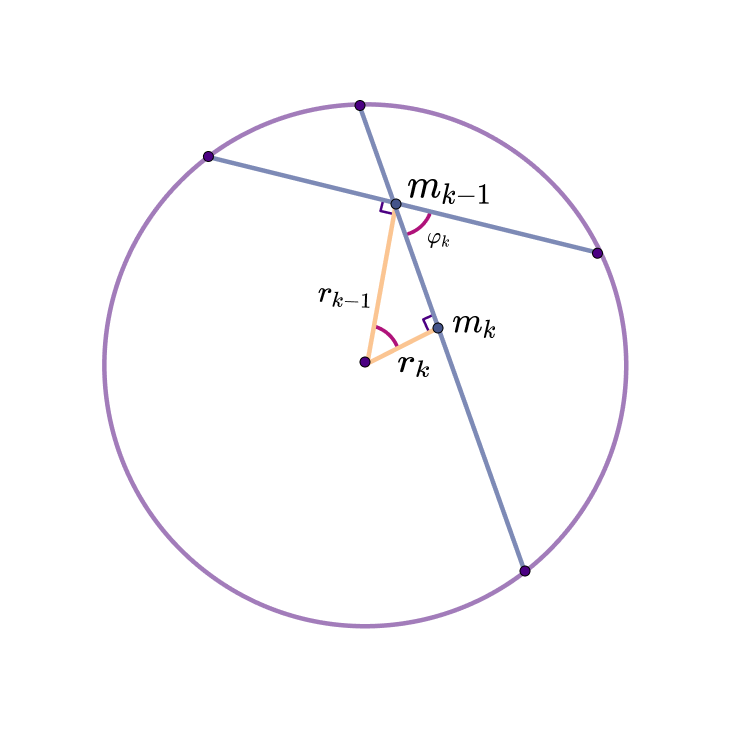
\includegraphics[width=0.4\textwidth]{Frame 1.png}
 \vspace{-5.5ex}
 
  \caption{Связь между приближениями $r_k$ и $r_{k-1}$.}
    \label{fig:sin_r}
\end{figure}


Если положить, что $\tau'_{\varepsilon} + 1 = \min\{k \geqslant  0 : r'_k \in S_\varepsilon\}$, то $\mathrm{E}_{\tau_{\varepsilon} +1}=\mathrm{E}_{\tau'_{\varepsilon} +1}$.

Получим, что:
\begin{equation}
\begin{aligned}
\left\{r_k^{\prime}<\varepsilon\right\}&=\left\{r_0 \prod_{i=1}^k \cos \varphi_i<\varepsilon\right\}=\left\{\sum_{i=1}^k \ln \cos \varphi _i <\ln \left(\varepsilon / r_0\right)\right\}\\
&=\left\{\sum_{i=1}^k-\ln  \cos \varphi_i >\ln \left(r_0 / \varepsilon\right)\right\}.
\end{aligned}
\label{eq:f_2}
\end{equation}

Обозначим $\mathrm{E}\ln \cos \varphi  =\mathrm{E} \ln \frac{r_k}{r_{k-1}}:= \mathrm{E}_{r}.$ Тогда $\mathrm{E}(-\ln \cos \varphi)=-\mathrm{E}_{r}>0.$\footnote{
Данное неравенство следует в силу значения $\mathrm{E}_{r}$, полученного в \ref{eq:f_8}.} 

Применяя теорему \ref{thm:е_1} с $t=\ln (r_0/\varepsilon) $ и $\mu(t)= \tau_{\varepsilon}+1$, получим, что имеет место следующая сходимость:\[
\frac{\mathrm{E}_{\tau_{\varepsilon} +1}}{\ln (r_0/\varepsilon)}\xrightarrow{\varepsilon \to 0 } \frac{1}{-\mathrm{E}_{r}}.
\]

Таким образом, среднее число шагов до достижения $S_\varepsilon$ растет очень медленно при $\varepsilon \to 0. $ 
\vspace{2ex}

Закончим оценку среднего количества шагов, вычислив $\mathrm{E}_{r}$.

Пусть $y=x_1^2$ -- квадрат первой координаты точки, отобранной равномерно случайным образом из $(n-1)$-сферы, тогда ее функция плотности вероятности для $y\in [0; 1]$ равна \cite{mardia2000directional}:
\begin{equation}
p(y)=\dfrac{\Gamma\left(\dfrac{n}{2}\right)}{\sqrt{\pi} \Gamma\left(\dfrac{n-1}{2}\right)}
(1-y)^{\frac{n-3}{2}}y^{-\frac{1}{2}}.
\label{eq:f_4}
\end{equation}

Обозначим $a=\dfrac{\Gamma\left(\frac{n}{2}\right)}{\sqrt{\pi} \Gamma\left(\frac{n-1}{2}\right)}$ и, используя \ref{eq:f_4}, получим формулу плотности для $x_1$:
\begin{equation}
\begin{aligned}
&\mathrm{P}(x_1<c)=\mathrm{P}(y<\sqrt{c})=a\int\limits_0^{\sqrt{c}}(1-y)^{\frac{n-3}{2}}y^{-\frac{1}{2}} \,dy = \\ & =  \left[\begin{array}{l}y=x_1^2\\ d y=2x_1 d x_1\end{array}\right]=2a\int\limits_0^{c}(1-x_1^2)^{\frac{n-3}{2}} \,dx_1.
\end{aligned}
\label{eq:dens}
\end{equation}
\vspace{0.5ex}

Тем самым $p_{x_1}$ имеет вид:
\begin{equation}
2a\cdot (1-x_1^2)^{\frac{n-3}{2}}.
\label{eq:dens_1}
\end{equation}
\newpage

Тогда необходимо вычислить следующий интеграл:
\begin{equation}
\begin{aligned}
   & \mathrm{E}_{r}= 2a \int\limits_0^1 (1-x_1^2)^{\frac{n-3}{2}}\ln(\sqrt{1-x_1^2})   \, d x_1 = a       
           \int\limits_0^1 (1-x_1^2)^{\frac{n-3}{2}}\ln(1-x_1^2)   \, d x_1 = \\
&= \left[\begin{array}{l}x_1 = \sin \varphi \\  d x_1= \cos \varphi \, d \varphi\end{array}\right] = 2a \int\limits_0^{\frac{\pi}{2}} (\cos \varphi)^{n-3}\cdot \ln \cos \varphi \cdot   \cos  \varphi \, d \varphi = \\ &= 2a \int\limits_0^{\frac{\pi}{2}} (\cos \varphi)^{n-2} \ln \cos \varphi \, d \varphi.
\end{aligned}
\label{eq:f_3}
\end{equation}


Известно \cite{gradshteyn}, что  $\displaystyle \mathrm{E}_{r'} = \int\limits_0^{\frac {\pi}{2}} (\cos \varphi)^{n-2} \ln \cos \varphi \, d\varphi: $ 
\begin{equation}
\displaystyle
\mathrm{E}_{r'}= \left\{\begin{array}{l}  -\dfrac{\pi}{2}\cdot \dfrac{(n-3)!!}{\sqrt{2}^{n-2}\left(\frac{n-2}{2}\right)!}\cdot \left[\ln 2 - \displaystyle \sum\limits_{i=1}^{n-2}\frac{(-1)^{i+1}}{i}\right],\; \, n-\text{четное},\\[3ex] 
\dfrac{\sqrt{2}^{n-3}\left(\frac{n-3}{2}\right)!}{(n-2)!!}\cdot \left[\ln 2 - \displaystyle \sum\limits_{i=1}^{n-2}\frac{(-1)^{i+1}}{i}\right],\; \, n-\text{нечетное}.
\end{array}\right.
\label{eq:f_5}
\end{equation}

Учтем, что:
\begin{equation}
a=\dfrac{\Gamma\left(\dfrac{n}{2}\right)}{\sqrt{\pi} \Gamma\left(\dfrac{n-1}{2}\right)}= \left\{\begin{array}{l} \displaystyle \dfrac{\sqrt{2}^{n-2}\left(\frac{n-2}{2}\right)!}{\sqrt{\pi}(n-3)!!} ,\; \, n-\text{четное},\\[2.5ex] 
\displaystyle \dfrac{(n-2)!!}{\sqrt{2}(n-3)!!} ,\; \, n-\text{нечетное}.
\end{array}\right.
\label{eq:f_6}
\end{equation}
\vspace{-1ex}

Объединяя \ref{eq:f_3}, \ref{eq:f_5} и \ref{eq:f_6}, получим, что искомое математическое ожидание:
\vspace{-4.5ex}

\begin{equation}
\displaystyle
\mathrm{E}_{r}= \left\{\begin{array}{l}  -\sqrt{\pi}\cdot  \left[\ln 2 - \displaystyle \sum\limits_{i=1}^{n-2}\frac{(-1)^{i+1}}{i}\right],\; \, n-\text{четное},\\[3ex] 
\dfrac{\sqrt{2}^{n-2}\left(\frac{n-3}{2}\right)!}{(n-3)!!}\cdot \left[\ln 2 - \displaystyle \sum\limits_{i=1}^{n-2}\frac{(-1)^{i+1}}{i}\right],\; \, n-\text{нечетное}.
\end{array}\right.
\label{eq:f_7}
\end{equation}
\vspace{-0.5ex}

Заметим, что так как при нечетном $n$ $n-3$ -- четное число, тогда двойной факториал можно представить в виде $(n-3)!!=2^{\frac{n-3}{2}}\left(\frac{n-3}{2}\right)!.$ 

Формула \ref{eq:f_7} примет вид:
\begin{equation}
\displaystyle
\mathrm{E}_{r}= \left\{\begin{array}{l}  -\sqrt{\pi}\cdot  \left[\ln 2 - \displaystyle \sum\limits_{i=1}^{n-2}\frac{(-1)^{i+1}}{i}\right],\; \, n-\text{четное},\\[3ex] 
\sqrt{2}\cdot \left[\ln 2 - \displaystyle \sum\limits_{i=1}^{n-2}\frac{(-1)^{i+1}}{i}\right],\; \, n-\text{нечетное}.
\end{array}\right.
\label{eq:f_8}
\end{equation}
\end{proof}

Отметим, что в формуле \ref{eq:f_8} $\ln 2$ --- это сумма знакочередующегося гармонического ряда, а $ \sum\limits_{i=1}^{n-2}\frac{(-1)^{i+1}}{i}$ --- его частичная сумма, то есть $\ln 2 -  \sum\limits_{i=1}^{n-2}\frac{(-1)^{i+1}}{i}$ --- остаток условно сходящегося ряда. Тем самым   $\mathrm{E}_{r}$ будет сходиться к нулю с увеличением размерности $n$, в силу того, что к нулю сходится остаток сходящегося ряда. 

Скорость сходимости к нулю остатка ряда является линейной, то есть с ростом $n$ каждый дополнительный член ряда уменьшает остаток на некоторую фиксированную величину. Тогда величина $ \displaystyle \dfrac{1}{-\mathrm{E}_{r}}$ при $n\to\infty$ будет сходиться к бесконечности, однако скорость, с которой это будет происходить, --- постоянная. 
%\newpage

Рассмотрим, чему равна константа $ \displaystyle \dfrac{1}{-\mathrm{E}_{r}}$, где $\mathrm{E}_{r}$ определяется формулой \ref{eq:f_8}, в зависимости от размерности пространства (Рис. \ref{fig:all_image7}). 

\begin{figure}[h]
  \centering
  \begin{subfigure}[b]{0.49\textwidth}
    \centering
    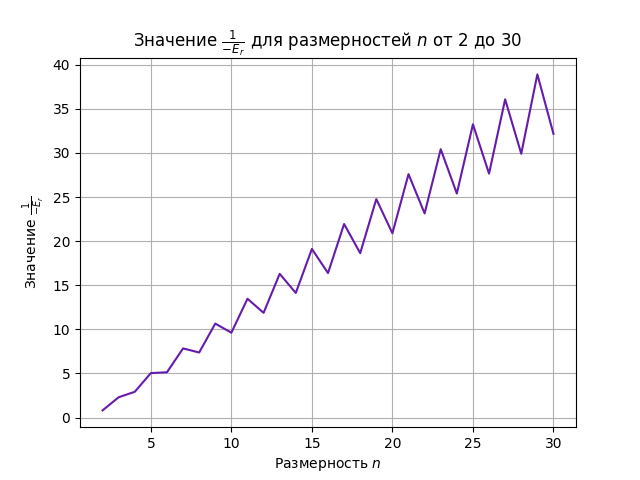
\includegraphics[width=\textwidth]{const30.png}
    \captionsetup{labelformat=empty}
     \caption{Размерности от $2$ до $30$}
  \end{subfigure}
  \begin{subfigure}[b]{0.49\textwidth}
    \centering
    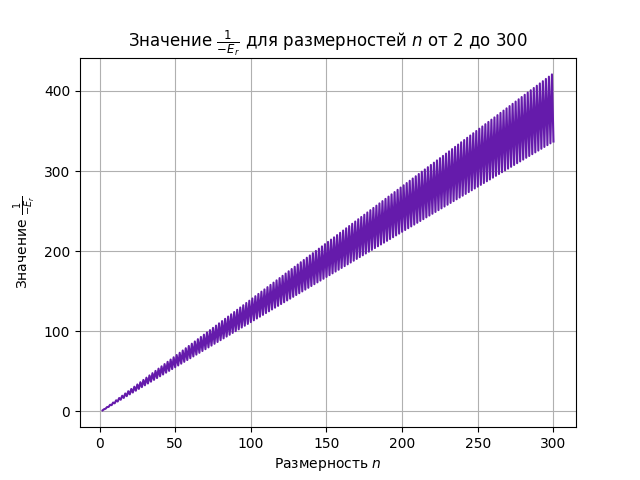
\includegraphics[width=\textwidth]{const300.png}
    \captionsetup{labelformat=empty}
    \caption{Размерности от $2$ до $300$}
  \end{subfigure}
   \caption{Значение константы $ \displaystyle \dfrac{1}{-\mathrm{E}_{r}}$ в зависимости от размерности. }
 \label{fig:all_image7}
\end{figure}

Таким образом, с увеличением размерности пространства алгоритм будет сходиться за большее количество шагов. При этом в случае нечетной размерности алгоритм будет сходиться быстрее, чем в случае четной. 
\newpage

\begin{corollary}
\label{col: c_1}
Теоретический доверительный интервал для математического ожидания количества шагов
\vspace{-3ex}

\begin{equation}
- x_{\alpha/2}  \sqrt{\dfrac{\ln (r_0/\varepsilon)\sigma^2}{-\mathrm{E}_{r}^3}} - \frac{\ln (r_0/\varepsilon)}{\mathrm{E}_{r}} < \mathrm{E}_{\tau_{\varepsilon} +1} <x_{\alpha/2}  \sqrt{\dfrac{\ln (r_0/\varepsilon)\sigma^2}{-\mathrm{E}_{r}^3}} - \frac{\ln (r_0/\varepsilon)}{\mathrm{E}_{r}}.
\label{eq:f_10}
\end{equation}
\end{corollary}
\begin{proof}

Чтобы применить теорему \ref{thm:е_2} для доказательства, необходимо вычислить дисперсию $\sigma^2=\mathrm{D}_r=\mathrm{E}_{r^2}-(\mathrm{E}_{r})^2$. 

Вычислив ее численно, на основе Рисунка \ref{fig:image_var} есть основание полагать, что $\sigma^2<\infty$, а значит можно применить  теорему \ref{thm:е_2} с $t=\ln (r_0/\varepsilon) $, $\mu(t)= \tau_{\varepsilon}+1$ и $a=-\mathrm{E}_{r}$.
\vspace{-4.5ex}

 \begin{figure}[h]
  \centering
  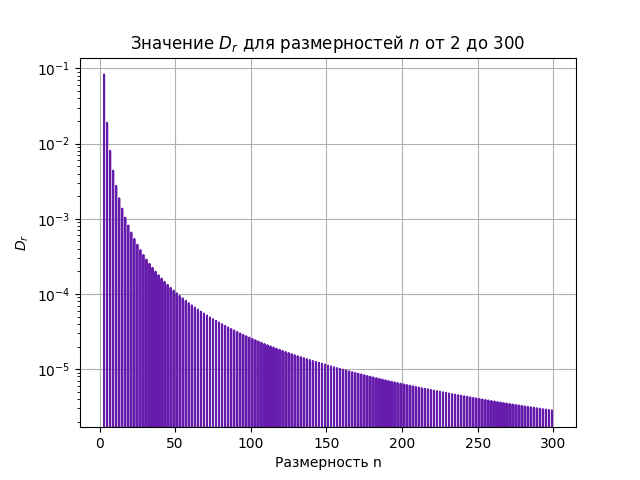
\includegraphics[width=0.52\textwidth]{varianse300.png}
  \caption{Дисперсия для размерностей от 2 до 300}
  \label{fig:image_var}
\end{figure}
\vspace{-2ex}

Тогда при $\varepsilon \to 0 $ получим, что имеет место следующая сходимость по распределению 
\[
\displaystyle \frac{\mathrm{E}_{\tau_{\varepsilon} +1} + \frac{\ln (r_0/\varepsilon)}{\mathrm{E}_{r}}}{\sqrt{\dfrac{\ln (r_0/\varepsilon)\sigma^2}{-\mathrm{E}_{r}^3}}}\xRightarrow{d} \mathrm{N}_{(0,1)}.
\]

Тем самым теоретический доверительный интервал для математического ожидания количества шагов
\begin{equation}
\left|\frac{\mathrm{E} (\tau_{\varepsilon}+1 ) + \frac{\ln (r_0/\varepsilon)}{\mathrm{E}_{r}}}{\sqrt{\dfrac{\ln (r_0/\varepsilon)\sigma^2}{-\mathrm{E}_{r}^3}}}\right|<x_{\alpha/2},
\label{eq:f_11}
\end{equation}
где $x_{\alpha/2}$ -- критическое значение стандартного нормального распределения, которое соответствует уровню значимости $\alpha/2$. 

Раскрывая модуль в формуле \ref{eq:f_11}, получим искомый результат \ref{eq:f_10}. 

\end{proof}

\chapter{Реализация и результат работы алгоритма}
\vspace{-0.5ex}

\section{Реализация}
\vspace{-1.5ex}

Приведем реализацию алгоритма~\ref{alg:median} на языке программирования Python.

\begin{lstlisting}[language=Python, caption={Функция, вычисляющая выборочную многомерную медиану}, label={lst:example}]
def find_median(sample, dimension, e=1.0e-2): 
    def generate_point_on_sphere(center):
        point = np.random.randn(dimension) 
        normalized_point = point / np.linalg.norm(point) 
        point_on_sphere =  center + normalized_point 
        return point_on_sphere

    def point_on_line(a, b, p): 
        ap = p - a
        ab = b - a
        result = a + np.dot(ap, ab) / np.dot(ab, ab) * ab
        return result

    def calc_approx_median(v, m, sample, sample_size): 
        proj = [point_on_line(v, m, sample[i]) for i in range(sample_size)]    
        m_next = np.median(proj, axis = 0)  
        return m_next

    sample_size = sample.shape[0]  
    m = sample[random.randrange(sample_size)] 
    v = generate_point_on_sphere(m)  
    mc = calc_approx_median(v, m, sample, sample_size)  
    while np.linalg.norm(m - mc) >= e:
        m = mc  
        v = generate_point_on_sphere(m)  
        mc = calc_approx_median(v, m, sample, sample_size)  

    return mc  
\end{lstlisting}

Данный код (Листинг \ref{lst:example}) представляет функцию \texttt{find_median}, которая используется для вычисления оценки некоторого многомерного обобщенного медианы  для выборки точек. Параметрами функции являются: \texttt{sample} --- выборка точек из распределения, соответствующего предположениям алгоритма~\ref{alg:median}; \texttt{dimension} --- размерность пространства, из которого взята выборка,  \texttt{e} --- точность вычисления. 

\begin{itemize}
\item \texttt{generate_point_on_sphere} --- это вспомогательная функция, которая генерирует точку, равномерно распределенную на единичной сфере в пространстве размерности \texttt{dimension}. Точка получается путем нормализации стандартной нормальной случайной величины. 

\item\texttt{point_on_line} --- это вспомогательная функция, которая вычисляет проекцию точки \textbf{p} на линию, заданную двумя точками \textbf{a} и \textbf{b}. Она использует векторную арифметику и скалярное произведение для получения проекции.

\item\texttt{calc_approx_median} --- это функция, вычисляющая приближенное значение медианы выборки \texttt{sample}. Она проецирует все точки выборки на прямую, определенную точками \textbf{v} и \textbf{m}, и находит медиану среди проекций. Затем вычисляется новая точка \textbf{m_next} на прямой, через которую будет проводиться прямая.
\end{itemize}

В основной части функции:
\begin{itemize}
\item\texttt{sample_size} получает количество точек в выборке \texttt{sample}.
\item\textbf{v} инициализируется случайной точкой на сфере, сгенерированной с помощью \texttt{generate_point_on_sphere}.
\item\textbf{m} устанавливается равным \texttt{sample[random.randrange(sample_size)] } (начальное приближение, выбранное случайным образом из точек выборки).
\item \textbf{mc} --- это первое приближение медианы с использованием \texttt{calc_approx_median} и начальных значений \textbf{v}, \textbf{m} и \texttt{sample}.
\end{itemize}

Цикл выполняется, пока \texttt{np.linalg.norm(m - mc) >= e} (расстояние между текущей медианой \textbf{m} и приближенной медианой \textbf{mc} больше или равно \texttt{e}). Если условие выполняется, \textbf{m} обновляется на \textbf{mc}, генерируется новая случайная точка на сфере \textbf{v}, и заново вычисляется \textbf{mc} с новыми значениями \textbf{v}, \textbf{m} и \texttt{sample}. Цикл продолжается до тех пор, пока разность не станет меньше или равна \texttt{e}.
\vspace{-1ex}

\section{Результат работы}

В результате работы функции (Листинг \ref{lst:example}) с $\varepsilon = 0{,}01$ для точек, равномерно распределенных в единичном круге, и для точек, имеющих  нормальное\footnote{Здесь и далее рассматривается нормальное распределение с такой же ковариационной матрицей $\scriptsize \begin{pmatrix}
1/4 & 0  \\
0 & 1/4
\end{pmatrix} $ и математическим ожиданием $(0 \;\;  0)^{\mathbf{T}}$ как и в случае равномерного распределения в круге, если не оговорено обратное.} распределение, получается следующий результат (Рис. \ref{fig:all_image1}). Зеленым изображены точки выборки из равномерного распределения в круге (Рис. \ref{fig:all_image1} a, b, c), сиреневым --- из нормального распределения (Рис. d, e, f). Градиентным красным отмечены приближения медианы, а темно-синим --- полученная оценка многомерной медианы. 

По графикам (Рис. \ref{fig:all_image1}) можно заметить, что независимо от объема выборки приближения сходятся к центру симметрии в случае обоих распределений. Это может говорить о том, что предложенный алгоритм действительно может использоваться для определения параметра положения. Также стоит отметить, что с увеличением объема выборки скорость сходимости увеличивается. 

Пусть теперь $70\%$ наблюдений из равномерного распределения в круге или из нормального, а  $30\%$ -- выбросы. Выбросами считаются точки, у которых компонента по $x$ имеет равномерное распределение на $(9{,}9; 10{,}1)$, а по $y$ -- нормальное  $\mathrm{N}_{(10,\ 0{,}1)}$. 


На основе данных графиков (Рис. \ref{fig:all_image2}) можно предположить, что при наличии выбросов алгоритм сходится примерно с такой же скоростью, но определяет параметр положения менее точно, чем в случае полного соответствия модели. 

Так как найденное значение близко к центру симметрии, есть основание полагать, что предложенная процедура является робастной.

\begin{figure}[h]
  \centering
  \begin{subfigure}[b]{0.4\textwidth}
    \centering
    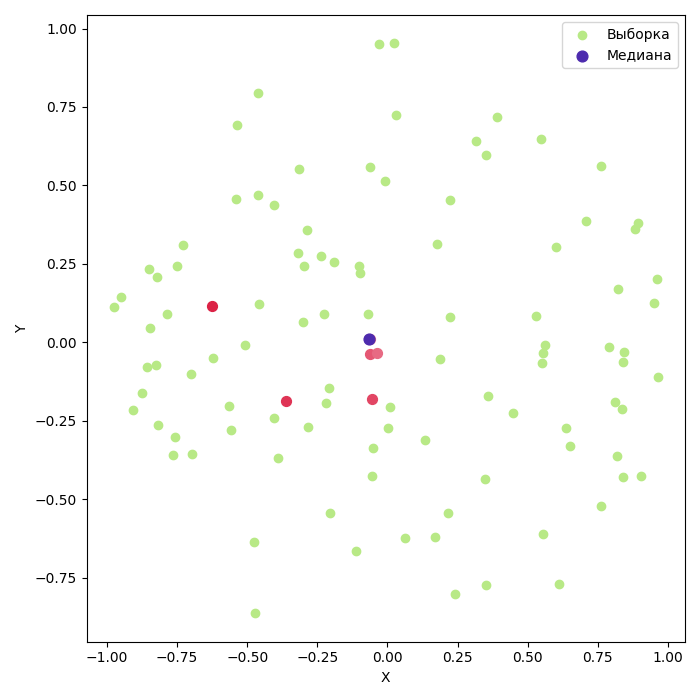
\includegraphics[width=\textwidth]{unif_circ_100.png}
    \captionsetup{labelformat=empty}
     \caption{(a) 100 точек}
     \label{fig:all_image1_a}
  \end{subfigure}
  \begin{subfigure}[b]{0.4\textwidth}
    \centering
    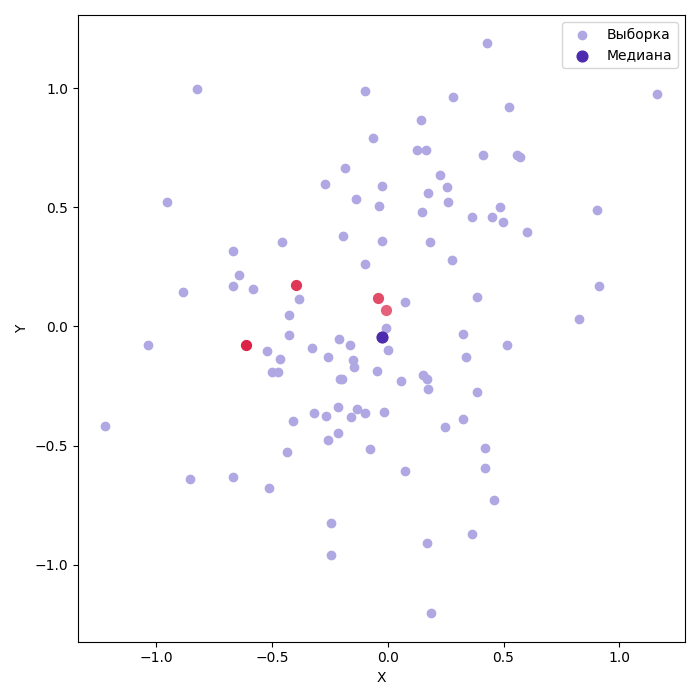
\includegraphics[width=\textwidth]{normal_100.png}
    \captionsetup{labelformat=empty}
    \caption{(d) 100 точек}
    \label{fig:all_image1_d}
  \end{subfigure}
  \begin{subfigure}[b]{0.4\textwidth}
    \centering
    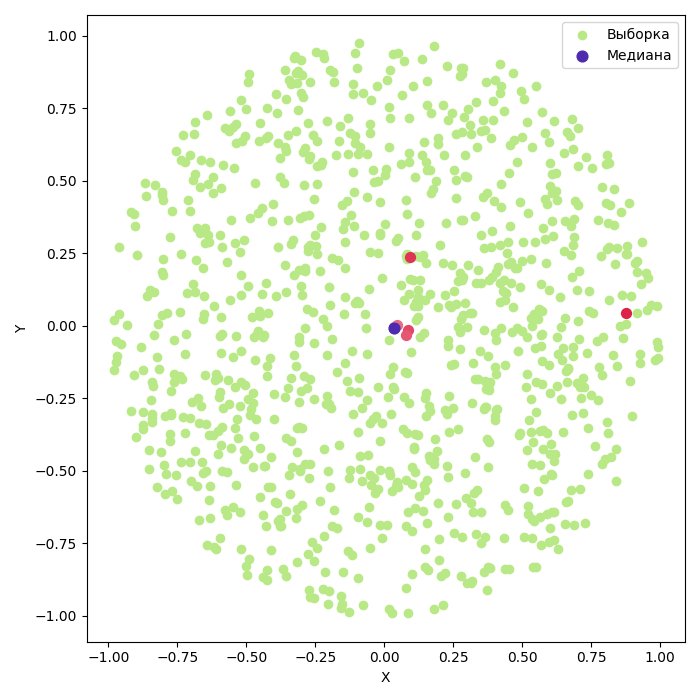
\includegraphics[width=\textwidth]{unif_circ_1000.png}
    \captionsetup{labelformat=empty}
     \caption{(b) 1000 точек}
     \label{fig:all_image1_b}
  \end{subfigure}
  \centering
  \begin{subfigure}[b]{0.4\textwidth}
    \centering
    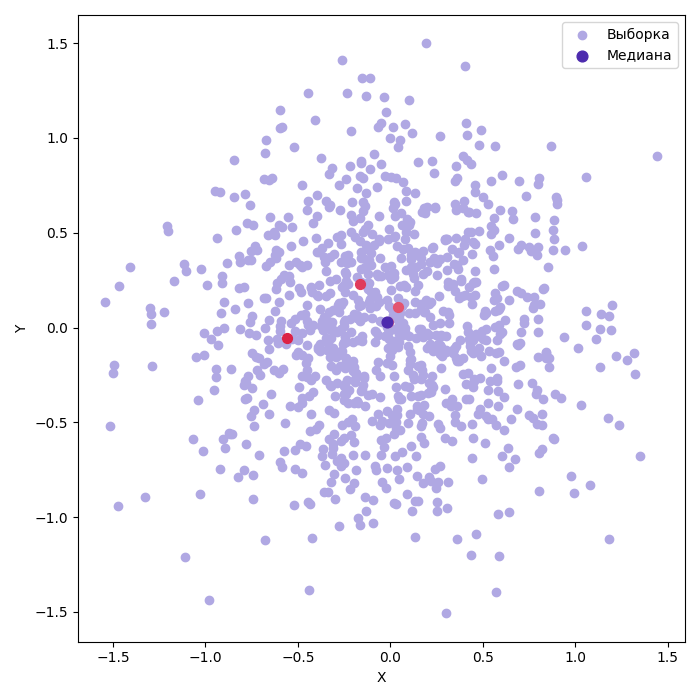
\includegraphics[width=\textwidth]{normal_1000.png}
    \captionsetup{labelformat=empty}
     \caption{(e) 1000 точек}
     \label{fig:all_image1_e}
  \end{subfigure}
  \begin{subfigure}[b]{0.4\textwidth}
    \centering
    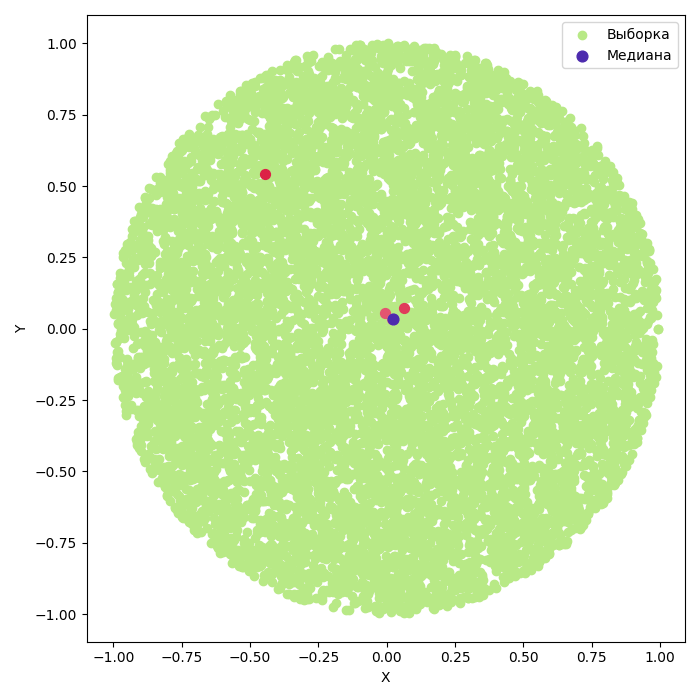
\includegraphics[width=\textwidth]{unif_circ_10000.png}
    \captionsetup{labelformat=empty}
    \caption{(c) 10000 точек}
    \label{fig:all_image1_c}
  \end{subfigure}
  \begin{subfigure}[b]{0.4\textwidth}
    \centering
    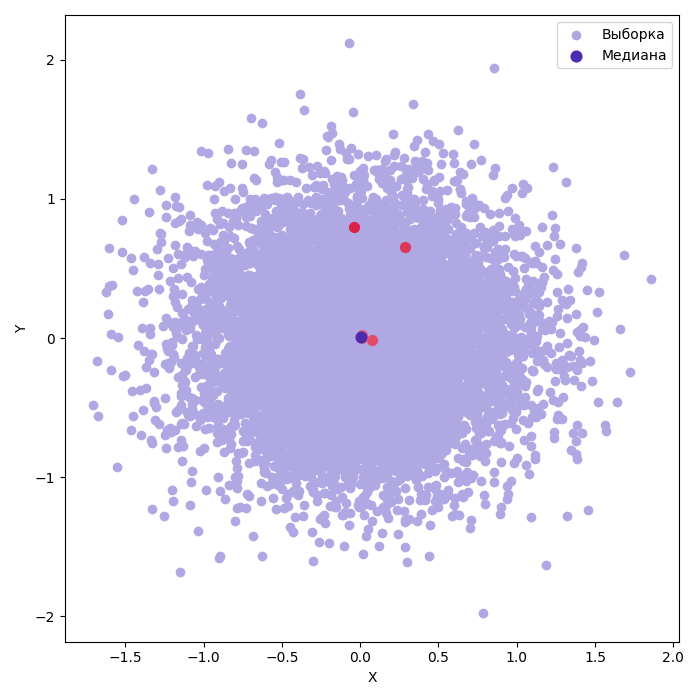
\includegraphics[width=\textwidth]{normal_10000.png}
    \captionsetup{labelformat=empty}
     \caption{(f) 10000 точек}
     \label{fig:all_image1_f}
  \end{subfigure}
  \caption{Результат работы алгоритма для разного объема выборок в случае равномерного в круге и нормального распределений }
 \label{fig:all_image1}
\end{figure}

\begin{figure}[h]
  \centering
  \begin{subfigure}[b]{0.4\textwidth}
    \centering
    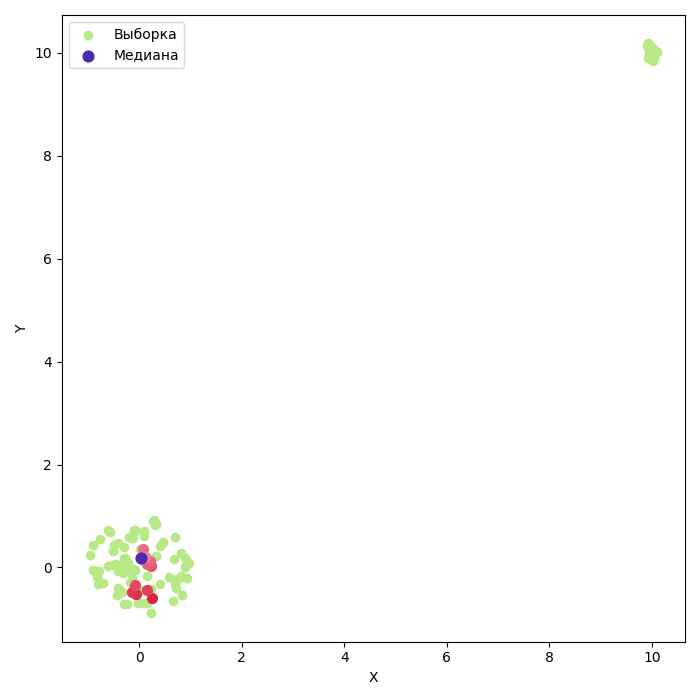
\includegraphics[width=\textwidth]{out_unif_circ_100.png}
    \captionsetup{labelformat=empty}
     \caption{(a) 100 точек}
  \end{subfigure}
  \begin{subfigure}[b]{0.4\textwidth}
    \centering
    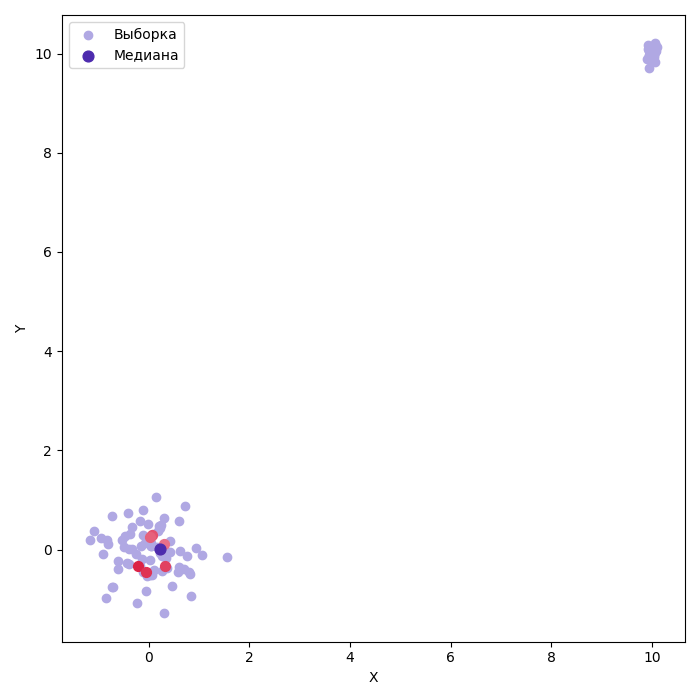
\includegraphics[width=\textwidth]{out_normal_100.png}
    \captionsetup{labelformat=empty}
    \caption{(d) 100 точек}
  \end{subfigure}
  \begin{subfigure}[b]{0.4\textwidth}
    \centering
    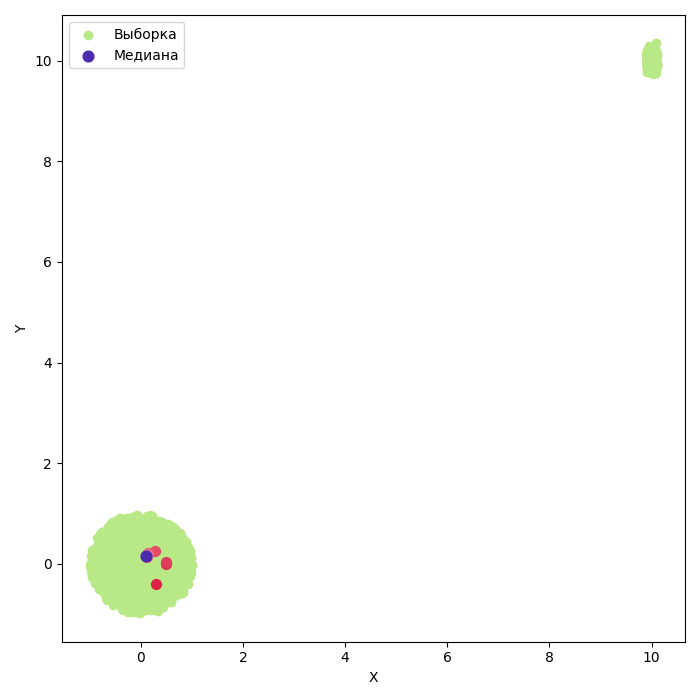
\includegraphics[width=\textwidth]{out_unif_circ_1000.png}
    \captionsetup{labelformat=empty}
     \caption{(b) 1000 точек}
  \end{subfigure}
   \centering
  \begin{subfigure}[b]{0.4\textwidth}
    \centering
    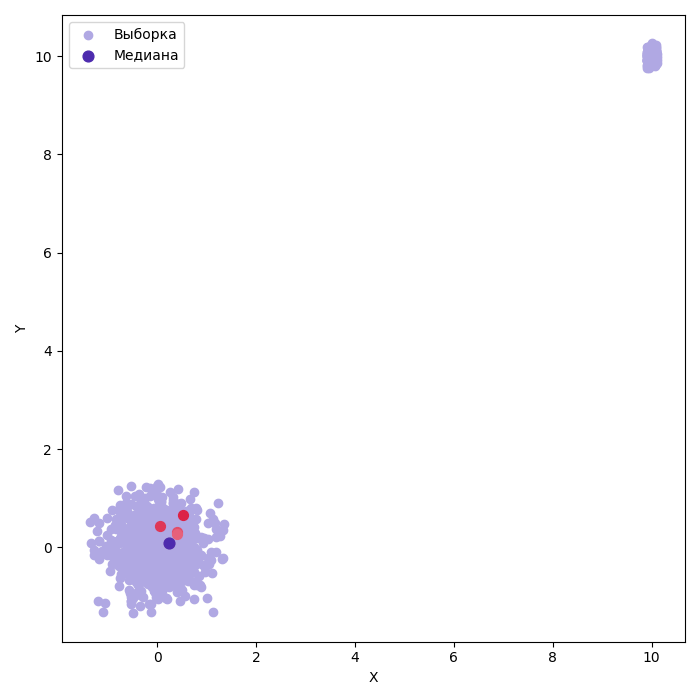
\includegraphics[width=\textwidth]{out_normal_1000.png}
    \captionsetup{labelformat=empty}
     \caption{(e) 1000 точек}
  \end{subfigure}
  \begin{subfigure}[b]{0.4\textwidth}
    \centering
    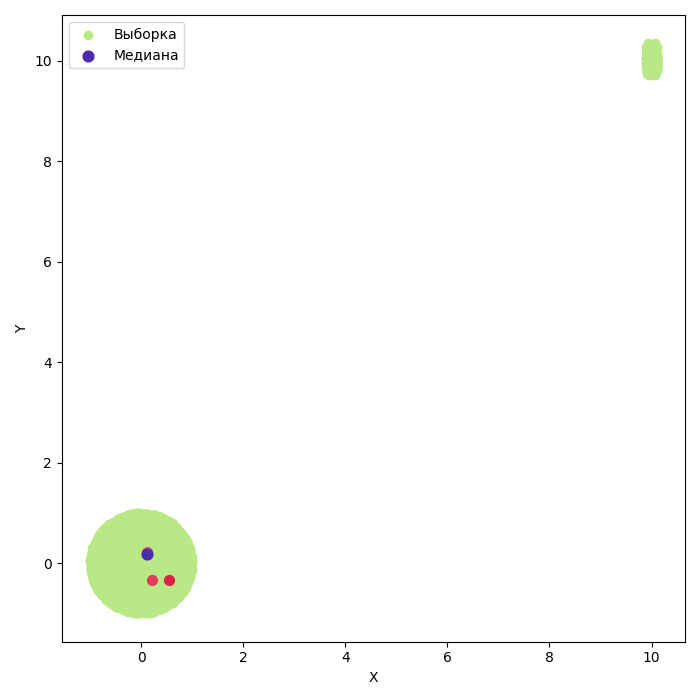
\includegraphics[width=\textwidth]{out_unif_circ_10000.png}
    \captionsetup{labelformat=empty}
    \caption{(c) 10000 точек}
  \end{subfigure}
  \begin{subfigure}[b]{0.4\textwidth}
    \centering
    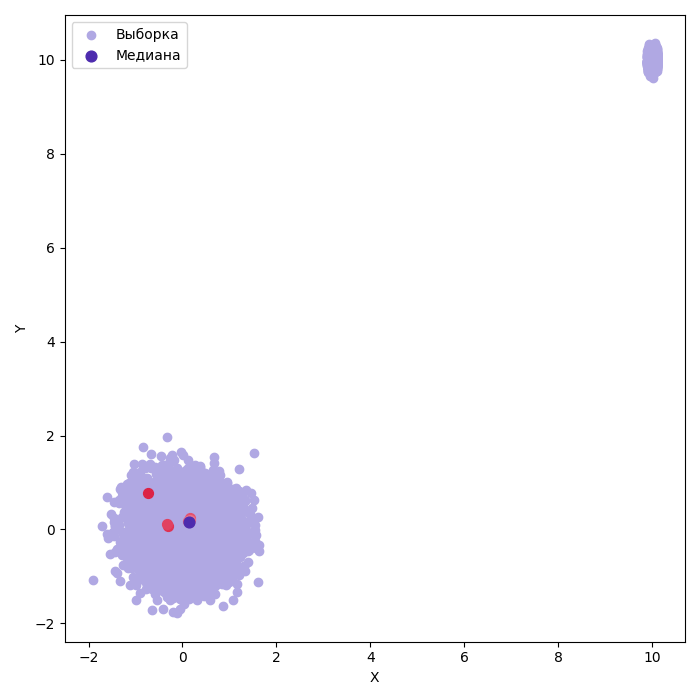
\includegraphics[width=\textwidth]{out_normal_10000.png}
    \captionsetup{labelformat=empty}
     \caption{(f) 10000 точек}
  \end{subfigure}
  \caption{Результат работы алгоритма для разного объема выборок с выбросами в случае равномерного в круге и нормального распределений}
 \label{fig:all_image2}
\end{figure}

\section{Сравнение результатов работы с другими алгоритмами}

Сравним работу алгоритмов для вычисления медиан Тьюки, Оджа \ref{eq:oja}, геометрической \ref{eq:spatial} и стохастической (Рис. \ref{fig:med_comp}).
\vspace{1ex}

\textbf{Сравнение в отсутствии выбросов}

Для начала рассмотрим изменение ошибки при увеличении объема выборки в случае равномерного распределения в круге (Рис. \ref{fig:med_comp} a). 

Новый стохастический алгоритм \ref{alg:median} показывает сопоставимые результаты с другими методами, при этом выигрывая в точности у своего конкурента по временной сложности -- геометрической медианы: при увеличении объема выборки стохастическая медиана дает более точные результаты, чем геометрическая. 
\vspace{0.5ex}

\textbf{Сравнение при наличии выбросов}

Рассмотрим теперь ситуацию, когда $30\%$ выборки из равномерного распределения заменена на выбросы, где выбросом считается точка на расстоянии 5 от истинного значения вес которой равен $30\%$ от объема выборки (Рис.  \ref{fig:med_comp} b).

Алгоритм \ref{alg:median} показывает более устойчивые результаты по сравнению с другими методами, демонстрируя меньшую чувствительность к выбросам. Даже при наличии выбросов значение ошибки остается относительно низким, что свидетельствует о его устойчивости и надежности в условиях загрязненных данных. 
\vspace{1ex}

Таким образом, на основе данных графиков есть основание полагать, что новый стохастический алгоритм \ref{alg:median} вычисления многомерной медианы является эффективным и устойчивым решением как для чистых, так и для загрязненных данных. 

\begin{figure}[h]
   \centering
\begin{subfigure}[b]{0.9\textwidth}
    \centering
    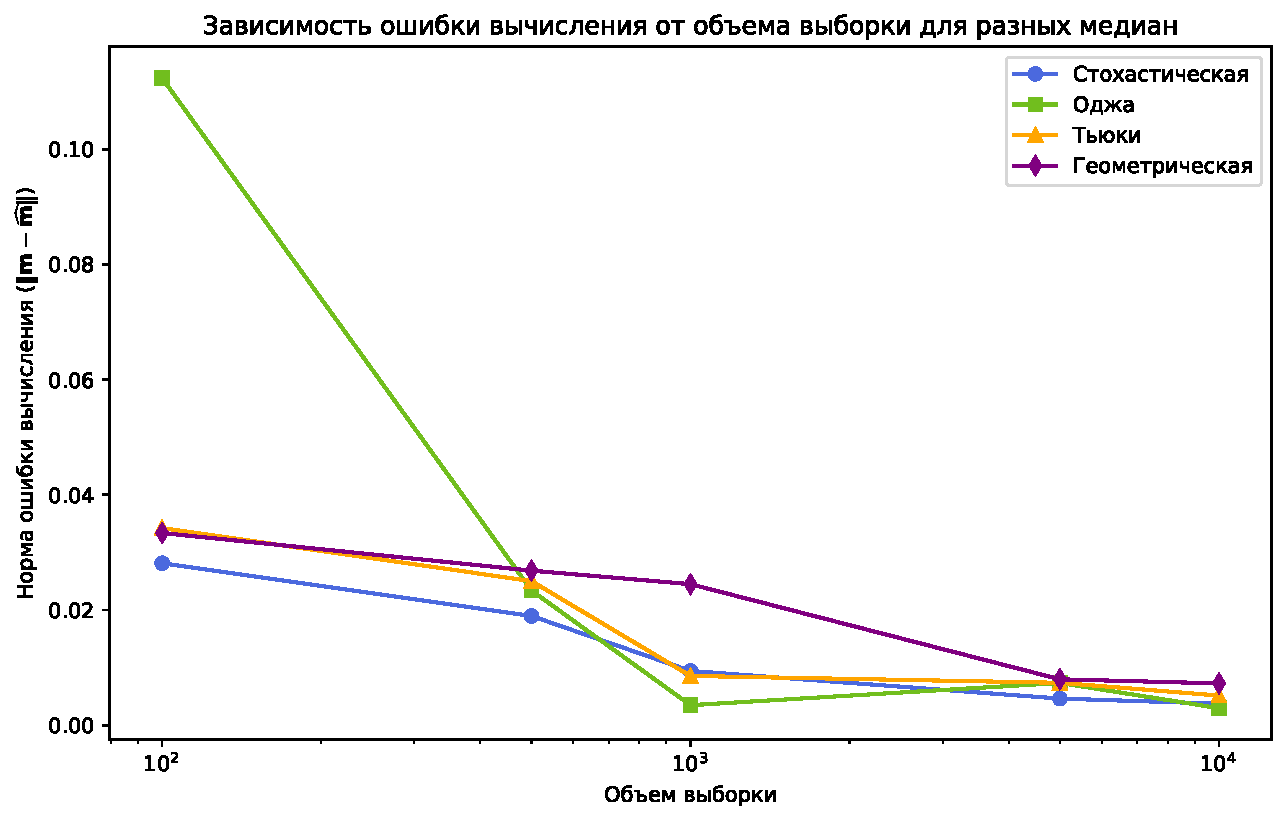
\includegraphics[width=\textwidth]{comp_unif.pdf}
    \captionsetup{labelformat=empty}
     \caption{(a) Равномерное}
        \label{fig:unif}
  \end{subfigure}
  \vspace{1ex}
  
  \begin{subfigure}[b]{0.9\textwidth}
    \centering
    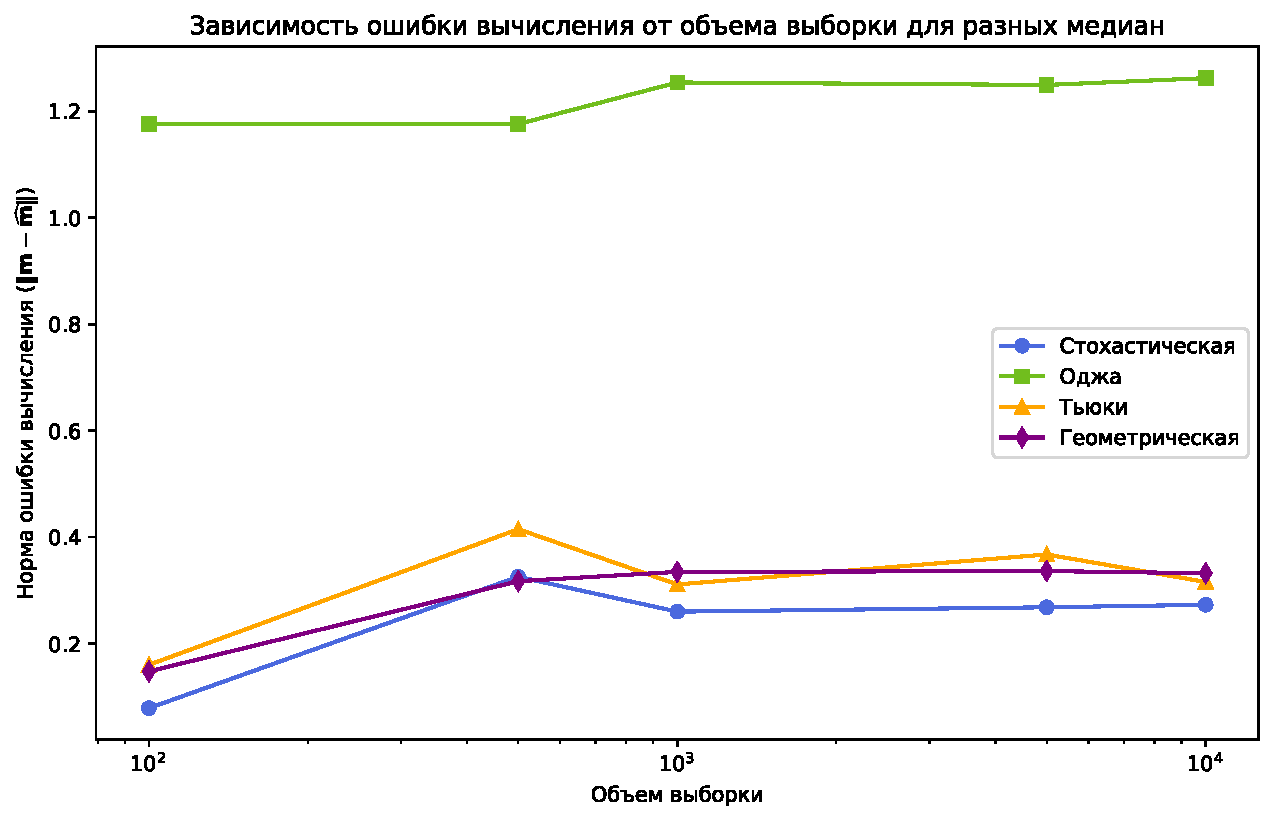
\includegraphics[width=\textwidth]{comp_unif_o.pdf}
    \captionsetup{labelformat=empty}
      \caption{(b) Равномерное с выбросами}
        \label{fig:unif_o}
  \end{subfigure}
  \caption{Рассматриваются выборки объемом 100, 500, 1000, 5000 и 10000 из равномерного распределения в круге с выбросами и без них. Для каждой выборки рассчитываются значения медиан Тьюки, Оджа, геометрической и стохастической.}
  \label{fig:med_comp}
\end{figure}


\chapter{Исследование сходимости и робастности}
\section{Сходимость}

\textbf{Зависимость нормы ошибки от количества итераций}

Для исследования скорости сходимости рассмотрим график (Рис. \ref{fig:image3}) зависимости нормы ошибки от количества итераций алгоритма. 

\begin{figure}[h]
    \centering
    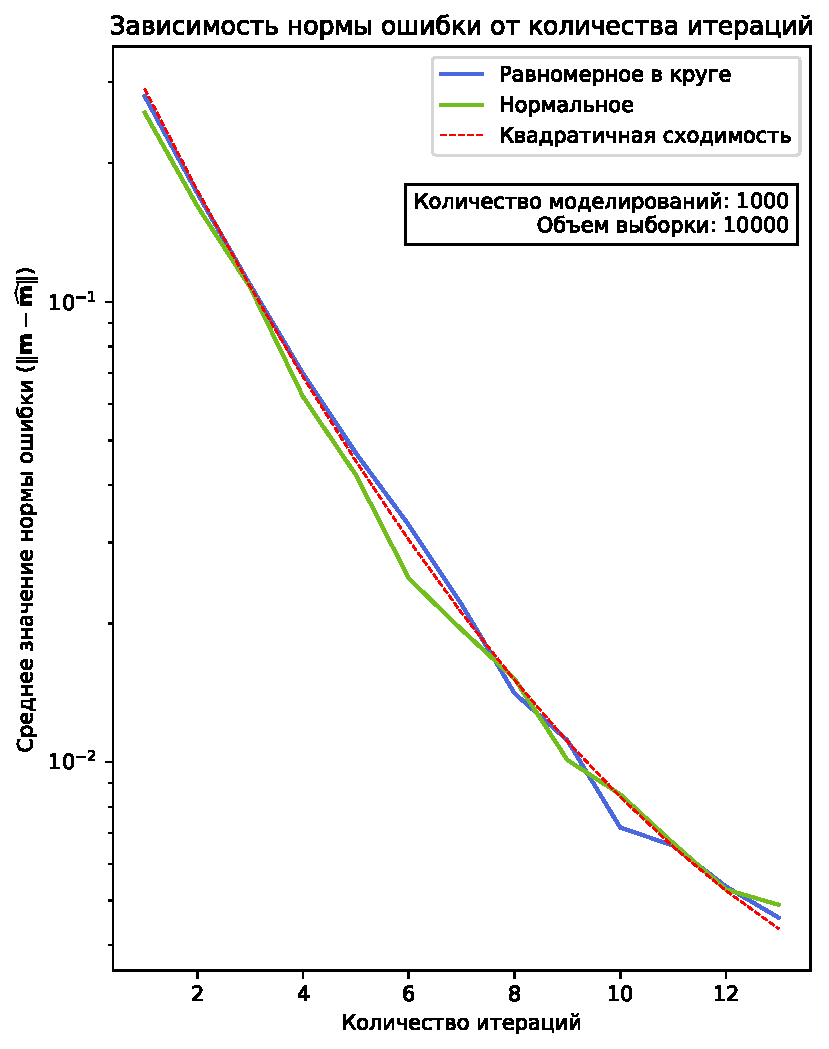
\includegraphics[width=0.65\textwidth]{mod_iter13_1000.pdf}
    \caption{Объем выборки 10000 и при заданном фиксированном количестве итераций $k$ делается 1000 моделирований, чтобы  получить среднее значение нормы ошибки, которая считается как разность между полученным значением $\widehat{\mathbf{m}}$ и истинным значением медианы $\mathbf{m}$ -- нулем. }
     \label{fig:image3}
\end{figure}
\vspace{-2ex}

Из Рисунка \ref{fig:image3} видно, что с увеличением количества итераций $k$ средняя ошибка существенно уменьшается для обоих распределений. 

На его основе можно предположить, что для пространства размерности 2 наблюдается близкая к квадратичной сходимость. Это означает, что ошибка уменьшается примерно как квадрат числа итераций. Квадратичная сходимость свидетельствует о высокой эффективности алгоритма~\ref{alg:median}, поскольку ошибка убывает очень быстро при увеличении числа итераций $k$. 

Этот результат имеет практическое значение, так как позволяет достигать значительной точности за малое количество итераций, существенно сокращая вычислительные затраты, особенно при анализе больших данных.
\vspace{1ex}

\textbf{Зависимость нормы ошибки от объема выборки}

Рассмотрим график (Рис. \ref{fig:image4}) зависимости нормы ошибки от объема выборки при фиксированном количестве итераций. 

\begin{figure}[h]
  \centering
  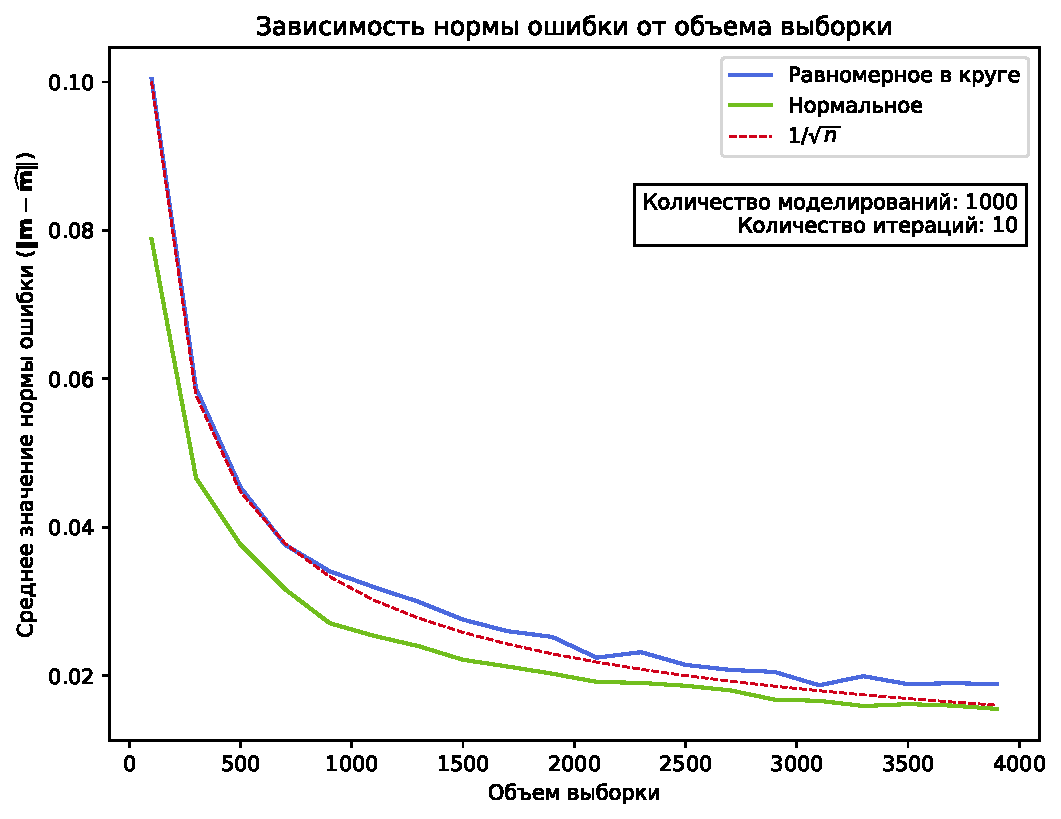
\includegraphics[width=0.8\textwidth]{mod_size_nor_uni.pdf}
  \caption{Исследуются выборки объемом от 100 до 4000 с шагом 100. При фиксированном количестве итераций $k=10$ для каждого объема выборки делается 1000 моделирований, чтобы получить среднее значение нормы ошибки. }
  \label{fig:image4}
\end{figure}
\vspace{-2ex}

Рисунок \ref{fig:image4} позволяет предположить, что при увеличении размера выборки, даже при небольшом количестве итераций, алгоритм~\ref{alg:median} демонстрирует более быструю сходимость к истинному значению. 

Более того, норма ошибки уменьшается почти как
$1/\sqrt{n}$, где $n$ -- объем выборки.
Это свидетельствует о том, что с ростом размера выборки ошибка уменьшается, но с убывающей скоростью. Если ошибка уменьшается данным образом, это может указывать на то, что увеличение размера выборки приводит к уменьшению дисперсии оценки.


Стоит отметить, что уменьшение ошибки в случае нормального распределения происходит немного быстрее, чем в случае равномерного распределения в круге. Это, вероятно, связано с более высокой вероятностью значений, близких к математическому ожиданию, в нормальном распределении, что обеспечивает более быструю сходимость к истинному значению. В равномерном распределении вероятность любого значения в пределах круга одинакова, что может потребовать большего числа итераций для достижения сходимости.
\vspace{1ex}

\textbf{Зависимость количества итераций алгоритма от точности}

Рассмотрим график (Рис. \ref{fig:image_eps}) зависимости среднего количества итераций алгоритма~\ref{alg:median} от значения точности~$\varepsilon$. 

		\begin{figure}[h]
			\centering
    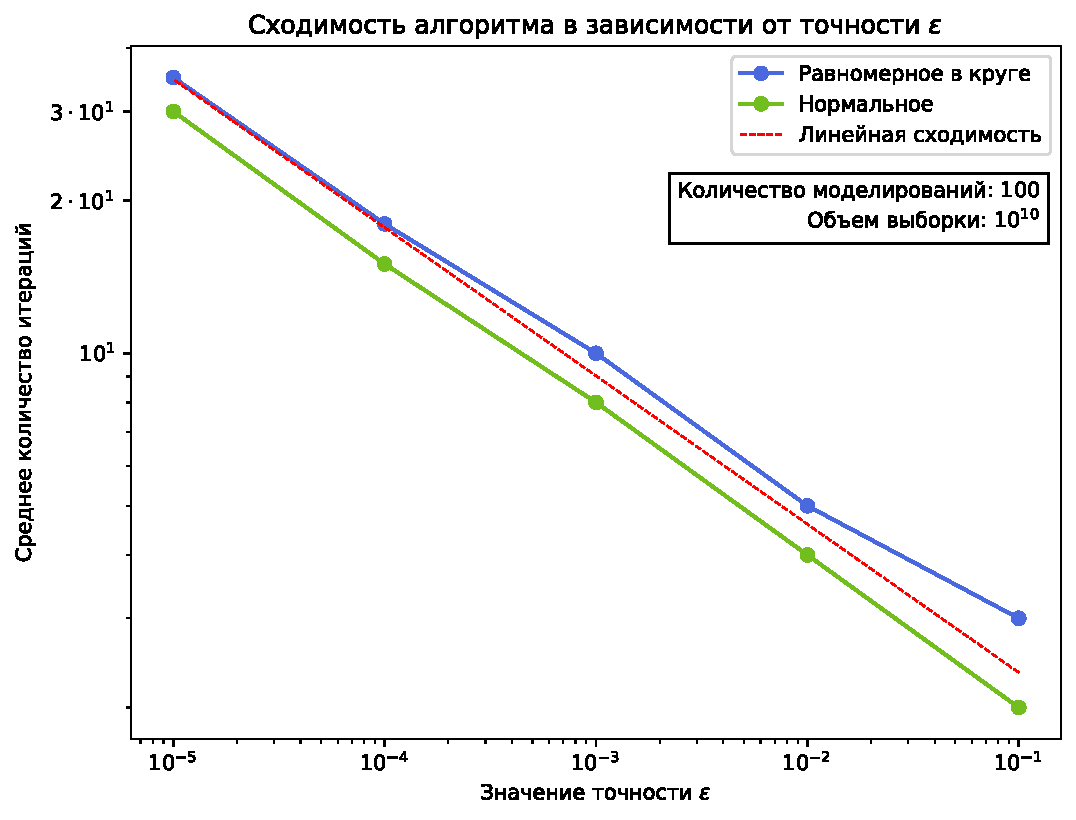
\includegraphics[width=0.8\textwidth]{eps_iter_1010.pdf}
        \caption{Рассматривается выборка объемом $10^{10}$ и значения точности от $0{,}1$ до~$0{,}00001$. При фиксированном значении $\varepsilon$ алгоритм запускается 100 раз и считается среднее количество итераций, за которое алгоритм достигнет заданной точности. }
			\label{fig:image_eps}
		\end{figure}
\vspace{-2ex}
 
Анализируя Рисунок \ref{fig:image_eps}, можно предположить, что между количеством итераций $k$, необходимых для достижения заданной точности $\varepsilon$, и значением самой точности существует экспоненциальная зависимость.

Это предположение кажется логичным по следующим причинам:
\vspace{-2ex}

\begin{enumerate}
    \item \textbf{Увеличение сложности с ростом точности}: с увеличением точности~$\varepsilon$ алгоритму~\ref{alg:median} требуется более тщательный поиск, что часто приводит к увеличению количества итераций $k$.
    
    \item \textbf{Уменьшение размера шага при увеличении точности}: с уменьшением значения $\varepsilon$ алгоритм~\ref{alg:median} должен точнее приближаться к истинному значению, что требует уменьшения шага на каждой итерации и увеличивает количество необходимых итераций.
\end{enumerate}
\vspace{-0.5ex}

\textbf{Зависимость нормы ошибки от количества итераций для разных размерностей}

Рассмотрим график (Рис. \ref{fig:all_image8}) зависимости нормы ошибки от количества итераций для равномерного распределения в шаре и для нормального с такой же ковариационной матрицей и математическим ожиданием в случае размерностей $2$-$6$.

\begin{figure}[h]
			\centering
    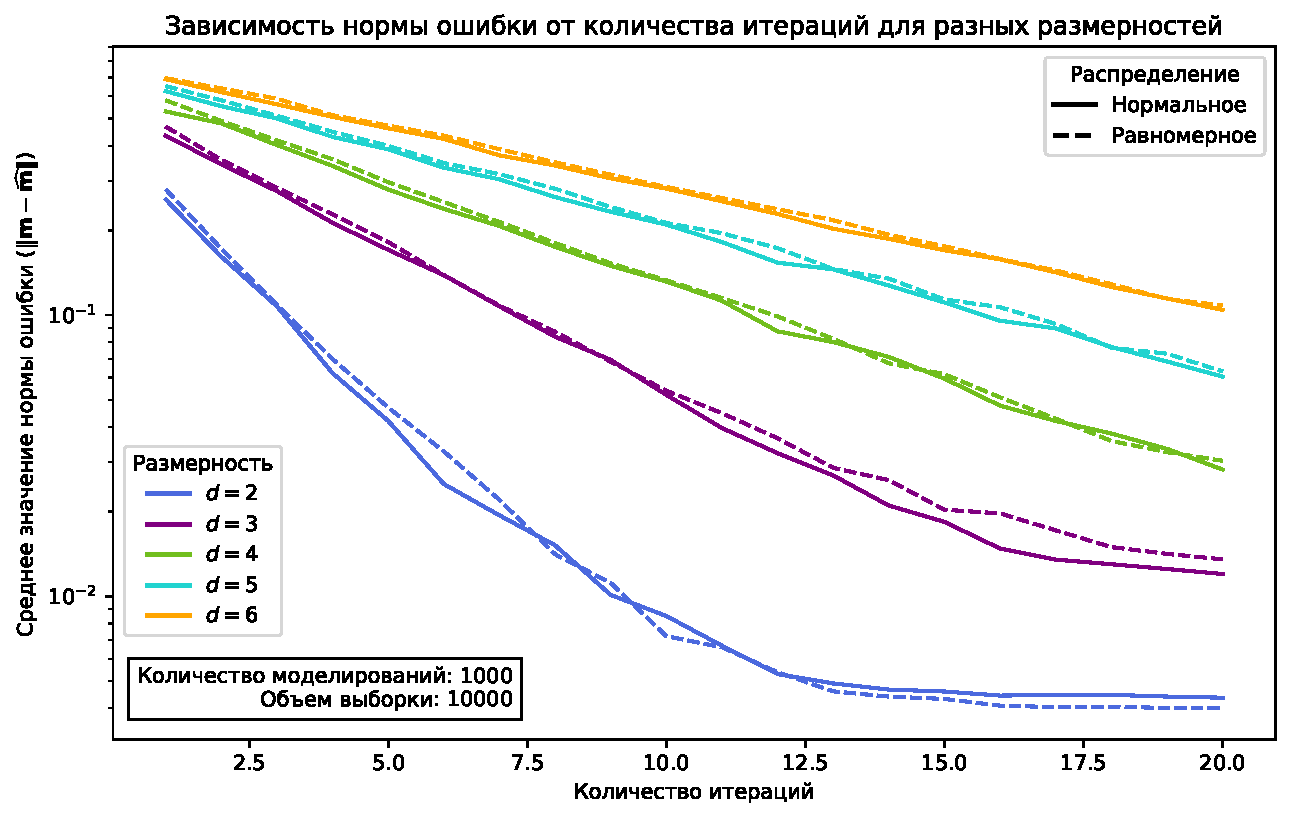
\includegraphics[width=0.9\textwidth]{mod_iter_1000_dim_normal_unif.pdf}
        \caption{Объем выборки 10000, точность $\varepsilon=0{,}01$, делается 1000 моделирований, чтобы  получить среднее значение нормы ошибки. }
			\label{fig:all_image8}
		\end{figure}
\vspace{-2ex}


Результаты моделирования (Рис. \ref{fig:all_image8}) показывают, что при увеличении размерности скорость сходимости алгоритма~\ref{alg:median} замедляется и приближение к истинному значению происходит за большее количество итераций. Причем это характерно для обоих рассматриваемых распределений в равной степени, то есть для равномерного и нормального распределения скорость уменьшения нормы ошибки с увеличением количества итераций $k$ примерно одинакова.  Это может говорить о том, что тип распределения оказывает незначительное влияние на общую тенденцию сходимости алгоритма~\ref{alg:median}.
 
 Более того, в случае размерностей $2,\ 3$ сходимость близка к квадратичной, а для размерностей $4-6$ она уже становится близкой к линейной. Это наблюдение является ожидаемым и обусловлено увеличением сложности задачи в многомерном пространстве. Однако как показывают результаты, небольшое изменение размерности не приводит к катастрофическому замедлению. Для размерностей $2-6$ алгоритм~\ref{alg:median} по-прежнему демонстрирует приемлемую скорость сходимости, несмотря на различия в характере уменьшения ошибки.

\section{Робастность}

\textbf{Добавление к выборке точки на заданном расстоянии от истинного значения}

Для начала рассмотрим результат работы алгоритма~\ref{alg:median} (Рис. \ref{fig:med_out_r}) в случае добавления к выборке из равномерного в круге и нормального распределений точек на заданном расстоянии от истинного значения. 

 Зеленым изображены точки выборки из равномерного распределения в единичном  круге (Рис. \ref{fig:med_out_r} a), сиреневым --- из нормального (Рис. \ref{fig:med_out_r} b), а цветные точки -- это приближения к медиане, полученные после добавления к выборке выброса на расстоянии $r$ от истинного значения параметра положения.

По Рисунку \ref{fig:med_out_r} можно сказать, что при наличии выбросов, удаленных на значительные расстояния от истинного значения медианы, алгоритм~\ref{alg:median} продолжает демонстрировать высокую точность приближений к этому значению. 

\newpage

\begin{figure}[h]
  \centering
\begin{subfigure}[b]{0.45\textwidth}
    \centering
    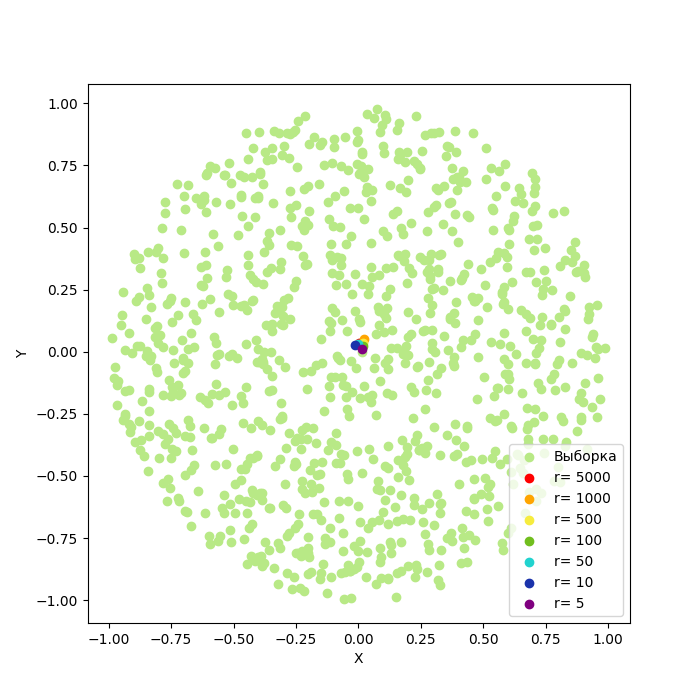
\includegraphics[width=\textwidth]{med_out_r_unif.png}
    \captionsetup{labelformat=empty}
     \caption{(a) Равномерное}
     \label{fig:unif_med}
  \end{subfigure}
  \begin{subfigure}[b]{0.45\textwidth}
    \centering
    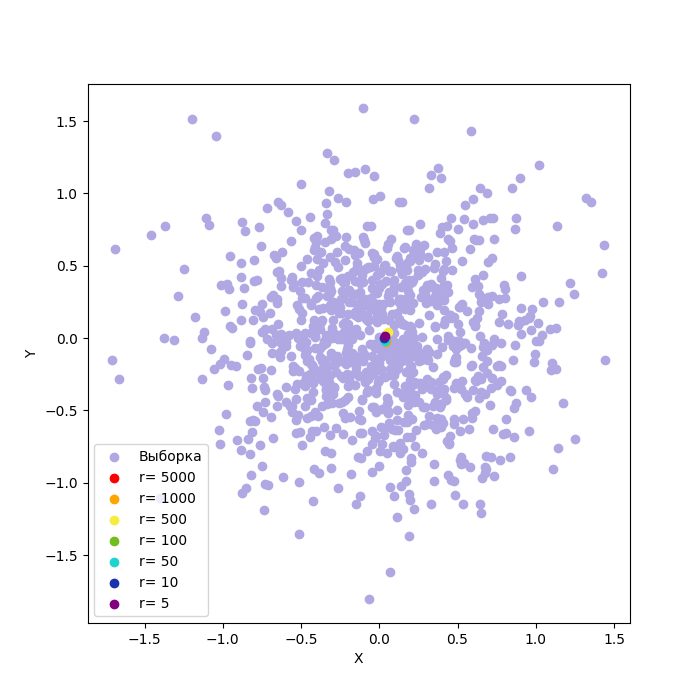
\includegraphics[width=\textwidth]{med_out_r_norm.png}
    \captionsetup{labelformat=empty}
    \caption{(b) Нормальное}
       \label{fig:normal_med}
  \end{subfigure}
   \caption{Рассматриваются выборки из равномерного в круге и нормального распределений объемом $1000$, к которым добавляется точка на расстоянии $5, \ 10, \ 50, \ 100,\ 500,\ 1000$ или $5000$ от истинного значения. Алгоритм запускается для $\varepsilon=0{,}01$.}
  \label{fig:med_out_r}
\end{figure}
\vspace{-3ex}

Устойчивость к добавлению выброса на различных расстояниях свидетельствует о конечности функции влияния \ref{eq:inf_fun} и ограниченности кривой чувствительности \ref{eq:SC_formula} для данной оценки.\footnote{Так как при вычислении стохастической медианы задача сводится к вычислению медианы на прямой, то можно оперировать понятиями главы 2, которые введены для одномерных данных.} Поскольку функция влияния \ref{eq:inf_fun} измеряет изменение оценки при добавлении загрязнения к распределению, а кривая чувствительности \ref{eq:SC_formula} оценивает изменение при добавлении отдельного наблюдения, ограниченные изменения оценки медианы при наличии выбросов демонстрируют, что алгоритм~\ref{alg:median} обладает низкой чувствительностью к большим выбросам и ограниченной функцией влияния. Это может свидетельствовать о робастности алгоритма~\ref{alg:median}  в присутствии выбросов.
\vspace{1ex}

\textbf{Добавление к выборке точки с весом на заданном расстоянии от истинного значения}

\textbf{Случай фиксированной точности}

Рассмотрим графики (Рис. $\ref{fig:med_out_m}$) зависимости нормы ошибки от веса выброса для различных расстояний от истинного значения.  
\newpage

\begin{figure}[h]
   \centering
\begin{subfigure}[b]{0.65\textwidth}
    \centering
    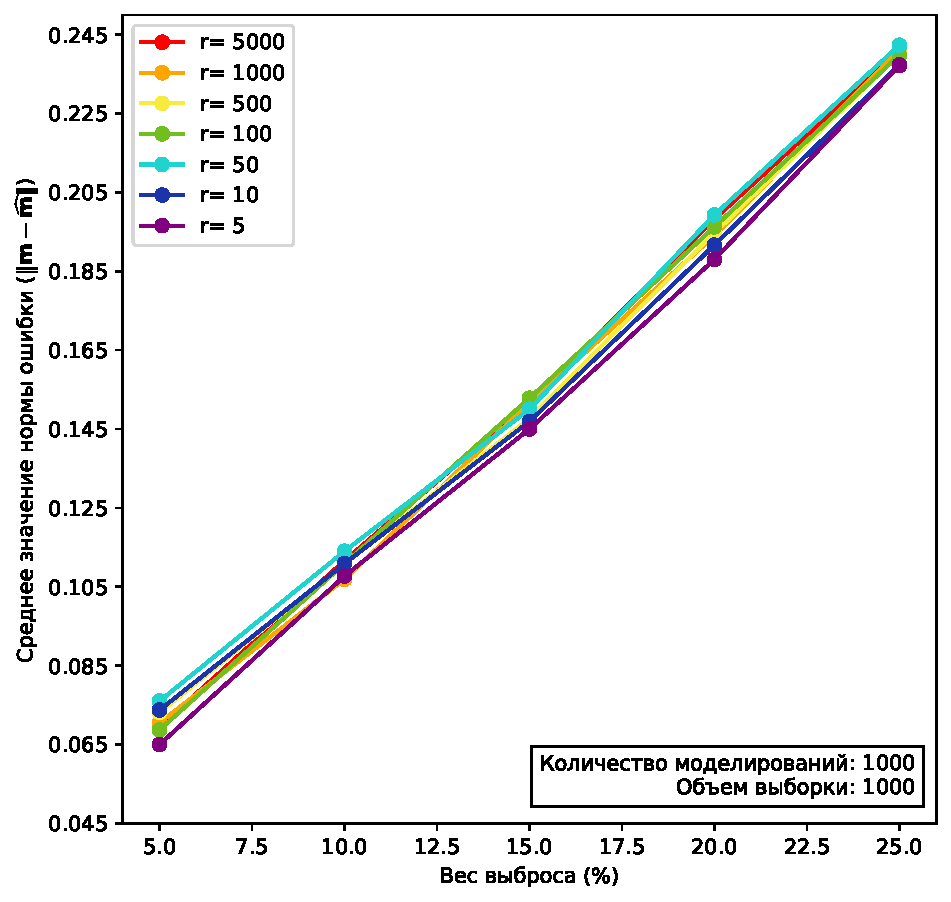
\includegraphics[width=\textwidth]{average_norm_vs_weight_unif.pdf}
    \captionsetup{labelformat=empty}
     \caption{ (a) Равномерное}
     \label{fig:aw_unif_e}
  \end{subfigure}
  \begin{subfigure}[b]{0.65\textwidth}
    \centering
    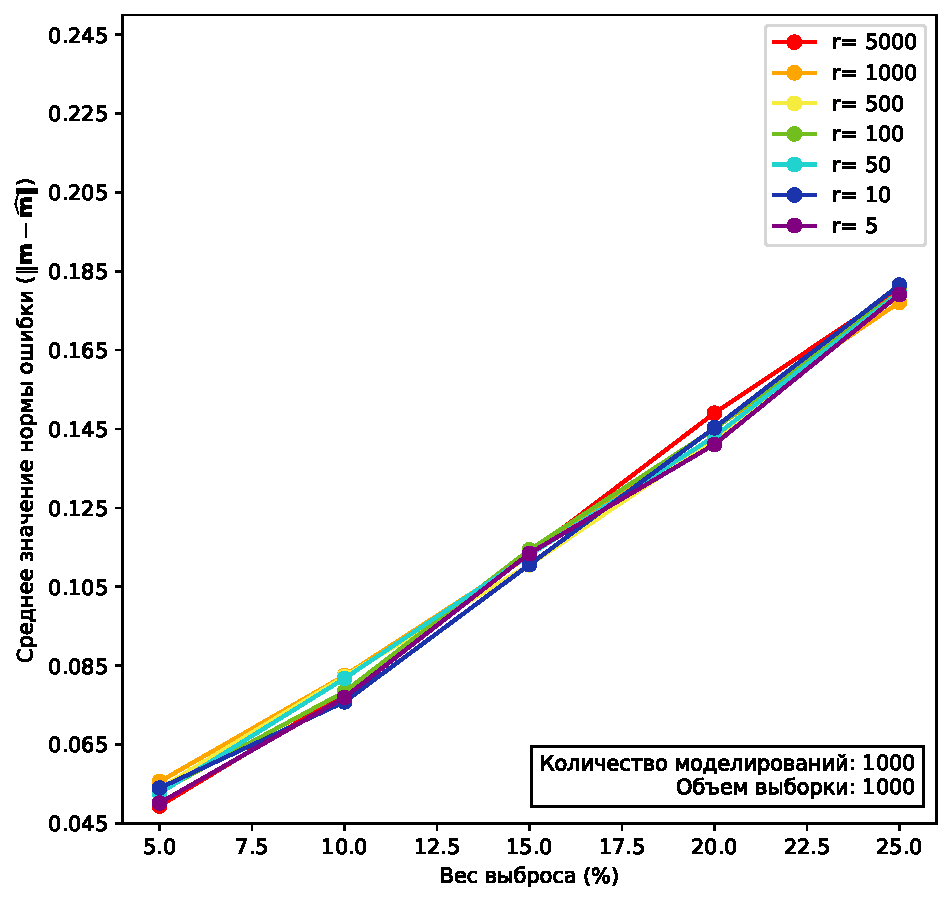
\includegraphics[width=\textwidth]{average_norm_vs_weight_norm.pdf}
    \captionsetup{labelformat=empty}
    \caption{(b) Нормальное}
     \label{fig:aw_normal_e}
  \end{subfigure}
  \caption{Рассматриваются выборки из равномерного в круге и нормального распределений объемом $1000$, к которым добавляется точка с заданным весом на расстоянии $r\in\{5, 10, 50, 100, 500, 1000, 5000\}$ от истинного значения.  Рассматриваются веса~$5\%,$ $10\%,\ 15\%,\ 20\%,\ 25\%$ от объема выборки. Алгоритм запускается для $\varepsilon=0{,}01$.  }
  \label{fig:med_out_m}
\end{figure}


Исходя из анализа Рисунка $\ref{fig:med_out_m}$, можно предположить, что точность оценки медианы уменьшается практически линейно с увеличением веса выброса. Это означает, что чем больше вес выброса, тем менее точной становится оценка. Причем от удаленности от истинного значения это не зависит, так как для всех~$r$ результаты примерно одинаковы при заданной точности $\varepsilon$. 

Таким образом, предполагается, что точность оценки медианы пропорциональна весу выброса, и при более значимых выбросах оценка становится менее точной. Причем в случае равномерного распределения точность оценки падает немного быстрее, при весе выброса около $15\%$ от объема выборки оценка становится недостаточно точной, чем в случае нормального распределения, где это происходит при весе выброса около $20\%$. 

Эта зависимость может быть объяснена пороговой точкой $\ref{eq:b_point_1}$, определяющей долю выборки, которую можно заменить выбросами, не нарушая робастность оценки. При превышении пороговой точки качество оценки ухудшается из-за слишком большого количества выбросов. Однако при наличии $25\% $ оценка хоть и не столь точна, но все же не находится на расстоянии, слишком далеком от истинного значения, поэтому можно предположить, что пороговая точка стохастической медианы не менее $0,25$. 

\vspace{1ex}

\textbf{Случай фиксированного количества итераций}

Рассмотрим графики, аналогичные Рисунку \ref{fig:med_out_m}, но в данном случае фиксируем количество итераций (Рис. $\ref{fig:med_out_m_fix}$) и на тех же данных запустим алгоритм. 

Исходя из анализа Рисунка \ref{fig:med_out_m_fix}, можно предположить, что удаленность выброса влияет на скорость сходимости алгоритма: для меньших значений $r$ алгоритм сходится быстрее, чем для больших значений $r$. 

При фиксированном количестве итераций при увеличении расстояния $r$ от истинного значения норма ошибки также увеличивается. Например, для выбросов, находящихся на расстоянии 5000 от истинного значения, норма ошибки составляет примерно 10 при весе выброса в $25\%$. В то же время, при фиксированной точности  норма ошибки остается низкой и не превышает 0,25. Это указывает на то, что при больших значениях $r$ требуется больше итераций для сходимости к истинной медиане. 

\begin{figure}[h]
   \centering
\begin{subfigure}[b]{0.75\textwidth}
    \centering
    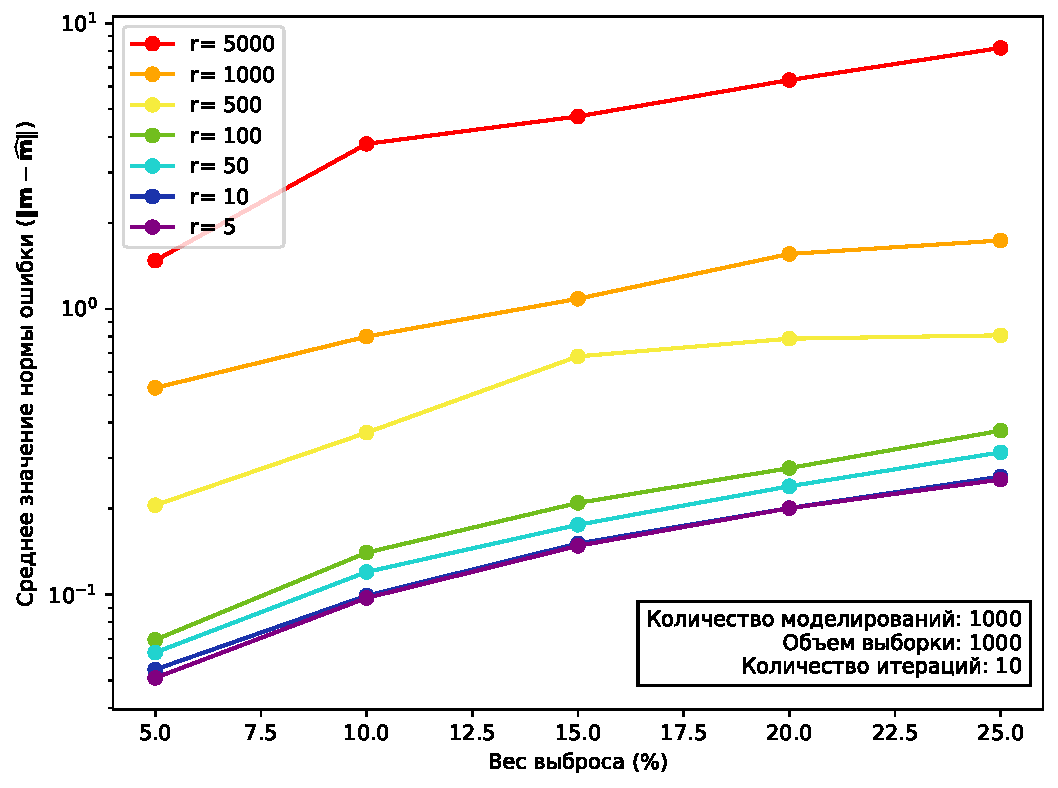
\includegraphics[width=\textwidth]{av_n_vs_w_unif.pdf}
    \captionsetup{labelformat=empty}
     \caption{(a) Равномерное}
     \label{fig:aw_unif}
  \end{subfigure}
  \begin{subfigure}[b]{0.75\textwidth}
    \centering
    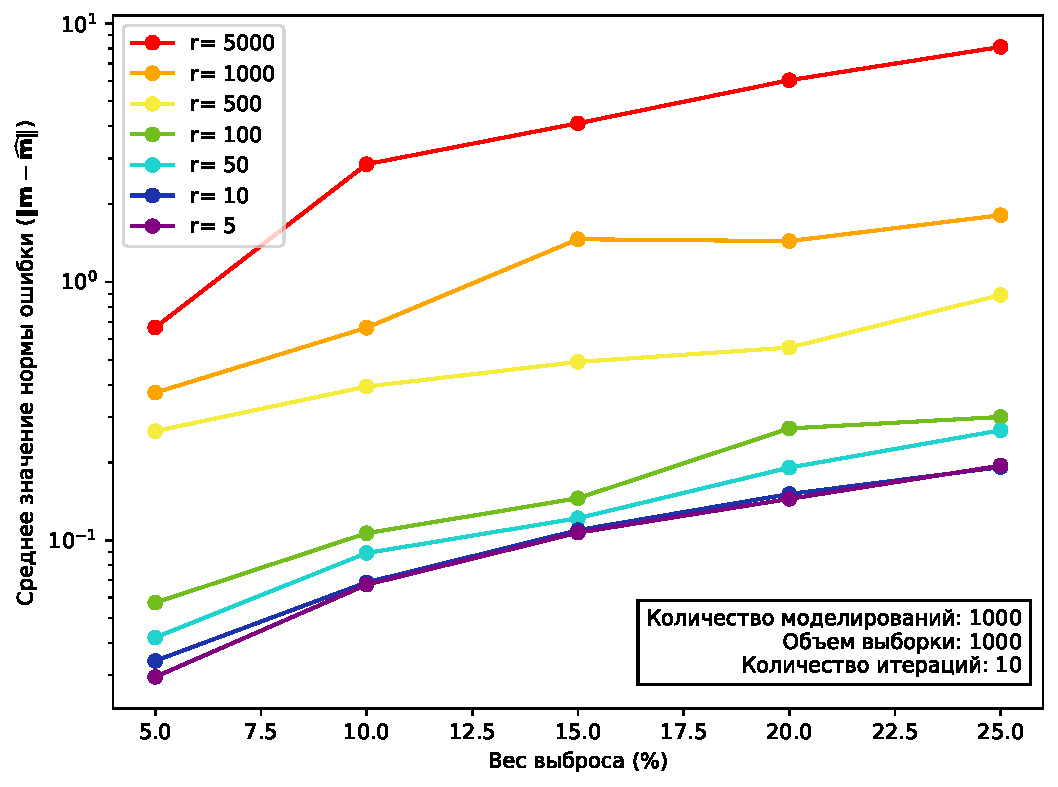
\includegraphics[width=\textwidth]{av_n_vs_w_norm.pdf}
    \captionsetup{labelformat=empty}
    \caption{(b) Нормальное}
      \label{fig:aw_normal}
  \end{subfigure}
  \caption{Рассматриваются выборки из равномерного в круге и нормального распределений объемом $1000$, к которым добавляется точка с заданным весом на расстоянии $r\in\{5, 10, 50, 100, 500, 1000, 5000\}$ от истинного значения.  Рассматриваются веса~$5\%,$ $10\%,\ 15\%,\ 20\%,\ 25\%$ от объема выборки. Алгоритм запускается для фиксированного количества итераций $k=10$.  }
  \label{fig:med_out_m_fix}
\end{figure}

\chapter{Исследование разброса оценки}

Для исследования разброса значений полученной оценки многомерного параметра положения для различных объемов $n\in \{ 100, 1000, 10000\}\, 1000$ раз моделировались выборки из заданного распределения. К каждой выборке был применен предложенный алгоритм~\ref{alg:median} при фиксированном количестве итераций $k=10$ и по полученным значениям было вычислено среднее значение $\boldsymbol{\mu}_n$ и выборочная ковариационная матрица $ \mathbf{\Sigma}_n$ для оценки медианы.  

Для равномерного распределения в единичном круге и для нормального распределения результаты следующие:

\begin{enumerate}
    \item \textbf{Равномерное в круге}
    
    \begin{itemize}
    \item $n=100$
    \[\small 
      \mathbf{\Sigma}_{100}=\begin{pmatrix}
6,51895e-03 & 3,16390e-04 \\
3,16390e-04 & 6,20397e-03 
\end{pmatrix}, \quad \boldsymbol{\mu}_{100}= \begin{pmatrix}
2,38430e-03  \\
-2,13803e-03
\end{pmatrix}.
    \]
    
    \item $n=1000$
    \[
    \small 
      \mathbf{\Sigma}_{1000}= \begin{pmatrix}
7,53798e-04 & 5,47668e-05  \\
5,47668e-05 & 8,53648e-04
\end{pmatrix}, \quad \boldsymbol{\mu}_{1000}=\begin{pmatrix}
-6,38330e-04  \\
-1,70367e-03
\end{pmatrix}.
    \]
    
    \item $n=10000$ 
    \[
    \small 
     \mathbf{\Sigma}_{10000}=
\begin{pmatrix}
1,40582e-04 & 1,07915e-05 \\
1,07915e-05 & 1,37997e-04
\end{pmatrix}, \quad \boldsymbol{\mu}_{10000}= \begin{pmatrix}
-1,02060e-04  \\
-2,12628e-05 
\end{pmatrix}.
    \]
\end{itemize}    

    \item \textbf{Нормальное}

        \begin{itemize}
    \item $n=100$
    \[
    \small 
       \mathbf{\Sigma}_{100}=\begin{pmatrix}
3,94001e-03 & 1,34764e-04 \\
1,34764e-04 & 3,82273e-03
\end{pmatrix}, \quad \boldsymbol{\mu}_{100}= \begin{pmatrix}
-2,81281e-03\\
-8,97540e-04
\end{pmatrix}.
    \]
    
    \item $n=1000$
    \[
    \small 
      \mathbf{\Sigma}_{1000}= \begin{pmatrix}
4,02848e-04 & 1,59198e-06  \\
1,59198e-06 & 4,15562e-04
\end{pmatrix}, \quad \boldsymbol{\mu}_{1000}=\begin{pmatrix}
1,29070e-04  \\
-8,72610e-04
\end{pmatrix}.
    \]
    
    \item $n=10000$ 
    \[
    \small 
    \mathbf{\Sigma}_{10000}=
\begin{pmatrix}
1,48952e-04 & 2,57817e-07 \\
2,57817e-07 & 1,27489e-04
\end{pmatrix}, \quad \boldsymbol{\mu}_{10000}= \begin{pmatrix}
2,14122e-04 \\ 
-2,58878e-05 
\end{pmatrix}.
    \]
\end{itemize}    
\end{enumerate}

С увеличением объема выборки оценка параметра становится точнее, что подтверждается приближением среднего значения к истинному центру симметрии распределений -- точке $(0 \;\;  0)^{\mathbf{T}}$ и уменьшением дисперсии. Для нормального распределения точность оценки выше, чем для равномерного, что видно из меньших значений ковариационной матрицы при одинаковом объеме выборки.

\vspace{0.5ex}

Рассмотрим доверительные эллипсоиды (Рис. \ref{fig:ellips}), построенные на основе полученных результатов.
\vspace{-0.5ex}

\begin{figure}[h]
  \centering
\begin{subfigure}[b]{0.45\textwidth}
    \centering
    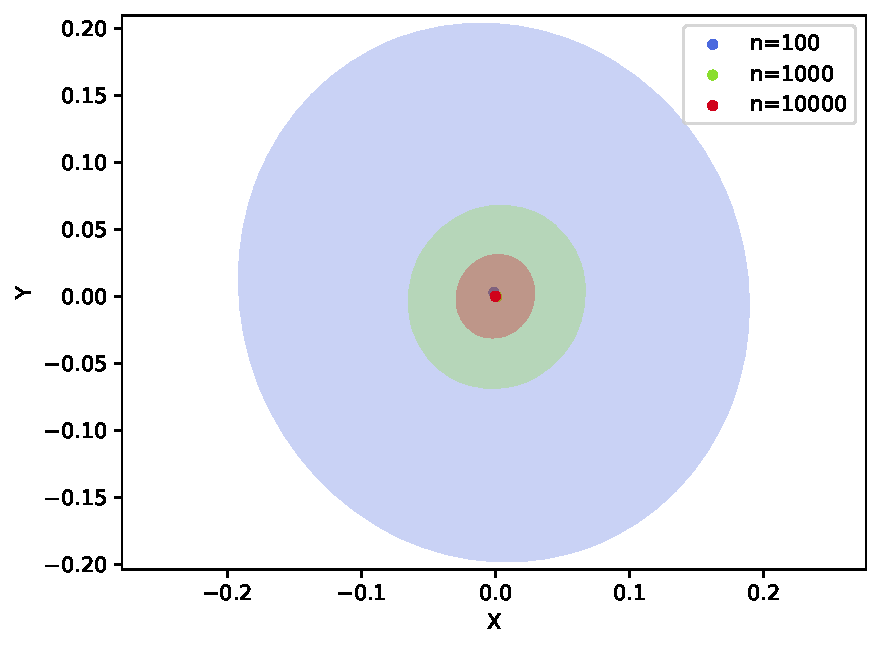
\includegraphics[width=\textwidth]{ellips_unif.pdf}
    \captionsetup{labelformat=empty}
     \caption{(a) Равномерное}
     \label{fig:el_unif}
  \end{subfigure}
  \begin{subfigure}[b]{0.45\textwidth}
    \centering
    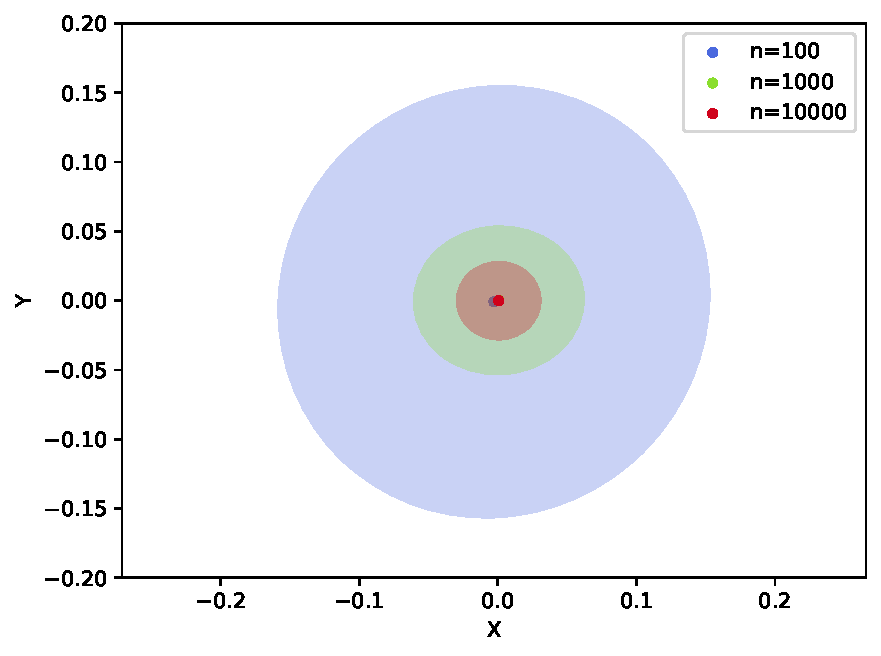
\includegraphics[width=\textwidth]{ellips_normal.pdf}
    \captionsetup{labelformat=empty}
    \caption{(b) Нормальное}
        \label{fig:el_normal}
  \end{subfigure}
  \vspace{-1ex}
  
   \caption{Доверительные эллипсоиды, построенные на основе полученных результатов для различных объемов выборки $n$. }
 \label{fig:ellips}
\end{figure}
\vspace{-2ex}

Доверительные эллипсоиды  (Рис. \ref{fig:ellips}) иллюстрируют разброс оценки параметра положения. 
Они строятся на основе ковариационных матриц $\mathbf{\Sigma}_n$  и отражают область, в которой с заданной вероятностью находится истинное значение параметра, в данном случае уровень доверия равен $95\%.$

 С увеличением объема выборки $n$ размер эллипсоидов уменьшается, что указывает на повышение точности оценок параметров положения. Для нормального распределения доверительные эллипсоиды оказываются меньше по размеру, чем для равномерного в круге, что указывает на большую точность и меньшую дисперсию оценок. 
 
Выводы на основе этих графиков (Рис. \ref{fig:ellips}) могут свидетельствовать об эффективности предложенного алгоритма \ref{alg:median} при оценке параметра положения.

\chapter{Заключение}

В данной работе во введении проведен обзор основных понятий робастности, ключевых для статистического анализа. Были рассмотрены кривая чувствительности, функция влияния и пороговая точка, которые важны для оценки степени робастности методов и понимания их поведения при наличии выбросов и других отклонений.

Центральным элементом исследования стал анализ нового робастного алгоритма оценивания многомерного параметра положения, в определенном смысле его можно рассматривать как обобщение медианы. Основными его достоинствами являются алгоритмическая простота и сопоставимость по точности и устойчивости с другими многомерными робастными оценками.

Важной задачей было изучение скорости сходимости предложенного алгоритма. Были проведены эксперименты и выполнен анализ результатов, что позволило сделать выводы о его эффективности и применимости в практических задачах. Особенно значимо, что была найдена скорость сходимости алгоритма в случае равномерного распределения в шаре, которая является экспоненциальной. 

Кроме того, работа алгоритма была сравнена с другими существующими методами. Результаты моделирования показали, что новый алгоритм не уступает конкурентам, особенно в условиях наличия выбросов.

В будущем возможны дальнейшие исследования и улучшения алгоритма, направленные на расширение его применимости и повышение эффективности. В частности, перспективными направлениями являются адаптация алгоритма для более сложных моделей данных.

Таким образом, проведенное исследование внесло определенный вклад в область робастного оценивания, предложив новый эффективный алгоритм и подтвердив его теоретическую и практическую ценность. 


%\addcontentsline{toc}{section}{Список литературы}
\bibliographystyle{ugost2008}
%\bibliographystyle{gost2008s}
\bibliography{bibliography}

\end{document}
